\usepackage{lipsum}
\usepackage{pdfpages} 
\begin{document}
\renewcommand{\figurename}{Figura}
\renewcommand{\tablename}{Tabela}
% =======================================================================================
%\cleardoublepage % Forces the first chapter to start on an odd page so it's on the right

% =======================================================================================
%                                   PREAMBLE
% =======================================================================================
\coverpage{\TITLE}{\SUBTITLE}{\AUTHOR}{\DATE}{\SUBJECT}
%----------------------------------------------------------------------------------------
% Blank Page----------------------------------------------------------------------------------------
\newpage
\thispagestyle{empty}
\mbox{}

% Blank Page----------------------------------------------------------------------------------------
\newpage
\thispagestyle{empty}
\mbox{}

% Blank Page----------------------------------------------------------------------------------------
\newpage
\thispagestyle{empty}
\mbox{}


\newpage
\section*{Equipe Responsável}
O trabalho foi conduzido sob a liderança de \textbf{Suhas Parandekar}, Economista Sênior. 
A equipe técnica foi composta por \textbf{Paulo Nascimento}, responsável pela dimensão de demanda de cursos técnicos; \textbf{Gabriel Grabowski}, responsável pela frente de oferta da Educação Profissional e Tecnológica (EPT); \textbf{Fábio Maciel}, responsável pelo desenvolvimento e análise de dados; e 
\textbf{Marina Bomura}, responsável pela coordenação e gestão do projeto.

Este relatório se beneficiou de discussões com outros membros da equipe do Banco Mundial para educação no Brasil, entre eles \textbf{Paulo Facundo Cuevas}, Economista-Líder; \textbf{Leandro Oliveira Costa}, Economista Sênior; \textbf{Ildo José Lautharte Júnior}, Economista Sênior; \textbf{Louisee Rodrigues da Cruz Boari}, Consultora Especialista em Educação; e \textbf{Isabella Miranda Meyer}, Associada Profissional Júnior.  O apoio administrativo foi prestado por \textbf{Débora Calheiros Fortes}.

A equipe trabalhou sob a orientação de \textbf{Andreas Blom}, Gerente de Prática de Educação do Banco Mundial para a Região da América Latina e Caribe.  
A \textbf{Diretora do Banco Mundial para o Brasil} é \textbf{Cécile Fruman}, e o \textbf{Diretor Global de Educação} é \textbf{Jaime Saavedra}.

A equipe é extremamente grata a \textbf{José Henrique Paim Fernandez}, Diretor da \textbf{Fundação Getulio Vargas – Diretoria de Desenvolvimento da Gestão Pública e Políticas Educacionais}, e à equipe da 
\textbf{FGV-DGPE} pela valiosa colaboração analítica e técnica.
Agradecemos, em especial, a \textbf{Aléssio Trindade} pelo apoio estratégico e pelas contribuições substanciais ao desenvolvimento do trabalho;  
a \textbf{Tullia Maria Erseni} pela coordenação e parceria constante;  
a \textbf{Carlos Ávila} e \textbf{Rogério Vidal} pelo suporte analítico na área de dados financeiros;  
e a \textbf{Garabed Kenchian} pelo apoio na análise de dados relacionados à Educação Profissional e Tecnológica (EPT).

A equipe expressa seu agradecimento ao \textbf{Ministério da Educação}, em especial à \textbf{Secretaria de Educação Profissional e Tecnológica (SETEC)} pelas conversas inicias sobre o PROPAG e ao \textbf{Instituto Nacional de Estudos e Pesquisas Educacionais Anísio Teixeira (MEC/INEP)}, bem como ao \textbf{Instituto Brasileiro de Geografia e Estatística (IBGE)} e ao \textbf{Instituto de Pesquisa Econômica Aplicada (IPEA)}, pelo fornecimento de informações estatísticas e socioeconômicas fundamentais para a análise e elaboração deste estudo.


\vspace{2em}

\textbf{Contactos:} sparandekar [at]  worldbank [dot]  org; 



\textbf{\textcolor{orange}{Plataforma Interativa na Internet:}}

\href{https://datanalytics.worldbank.org/content/6604f317-d487-436a-b6b6-792369b341f0}{https://datanalytics.worldbank.org/Plataforma Interativo PROPAG} 


% Blank Page----------------------------------------------------------------------------------------
\newpage
\thispagestyle{empty}
\mbox{}


\newpage
\cleardoublepage
\thispagestyle{empty}

\vspace*{6cm}

\begin{center}
	{\LARGE \textbf{Em Memória}}
	
	\vspace{1cm}
	
	{\large
		Expressamos nosso profundo pesar pelo falecimento de \textbf{Gabriel Grabowski},\\
		que integrou esta equipe com dedicação exemplar e contribuições fundamentais para\\
		a Educação Profissional e Tecnológica no Brasil.
		
		\vspace{0.5cm}
		
		Seu trabalho, compromisso e espírito colaborativo permanecerão como inspiração\\
		para todos os que tiveram a honra de com ele conviver.
	}
	
	\vspace{1.5cm}
	
	{\normalsize
		\textit{Com reconhecimento e gratidão,\\
			a equipe deste estudo.}
	}
\end{center}


% Blank Page----------------------------------------------------------------------------------------
\newpage
\thispagestyle{empty}
\mbox{}

% TOC

\newpage
\tableofcontents
\clearpage


\newpage
\part{Introdução e Contexto}

% Blank Page----------------------------------------------------------------------------------------
\newpage
\thispagestyle{empty}
\mbox{}


\chapter{Introdução} \label{ch:intro}
%\addcontentsline{toc}{section}{Introdução}
O objetivo deste relatório é fornecer bases analíticas com evidências empíricas como um de vários insumos para o desenvolvimento de políticas de Educação Profissional e Tecnológica (EPT) no contexto do PROPAG. A \href{https://datanalytics.worldbank.org/content/6604f317-d487-436a-b6b6-792369b341f0}{Plataforma Analítica Juros por Educação do BM--FGV} organiza estas análises em cinco dimensões fundamentais: (A) contexto demográfico e populacional; (B) cenários financeiros e simulações do PROPAG; (C) oferta atual e projetada de EPT; (D) demanda por formação técnica com base no desenvolvimento econômico regional; e (E) análise integrada entre oferta e demanda. A ferramenta permite ao usuário explorar dados detalhados de sua unidade federativa, realizar comparações entre estados e regiões, e simular diferentes cenários de adesão ao programa, oferecendo assim um conjunto robusto de informações para a definição de políticas sobre a expansão da EPT como fator importante para aumentar a produtividade do trabalhador no Brasil.

\begin{center}
	\textbf{\textcolor{orange}{Plataforma Interativo na Internet:}}\\
	\href{https://datanalytics.worldbank.org/content/6604f317-d487-436a-b6b6-792369b341f0}{https://datanalytics.worldbank.org/Plataforma-Interativo-PROPAG}
\end{center}

\section{Navegação da Plataforma}

A plataforma está estruturada em \textbf{múltiplas abas temáticas}, cada uma voltada a um aspecto crítico para a tomada de decisão. A interface principal, ilustrada na Figura~\ref{fig:intro_page}, apresenta todas as dimensões de análise organizadas de forma intuitiva.

\begin{figure}[htbp]
	\centering
	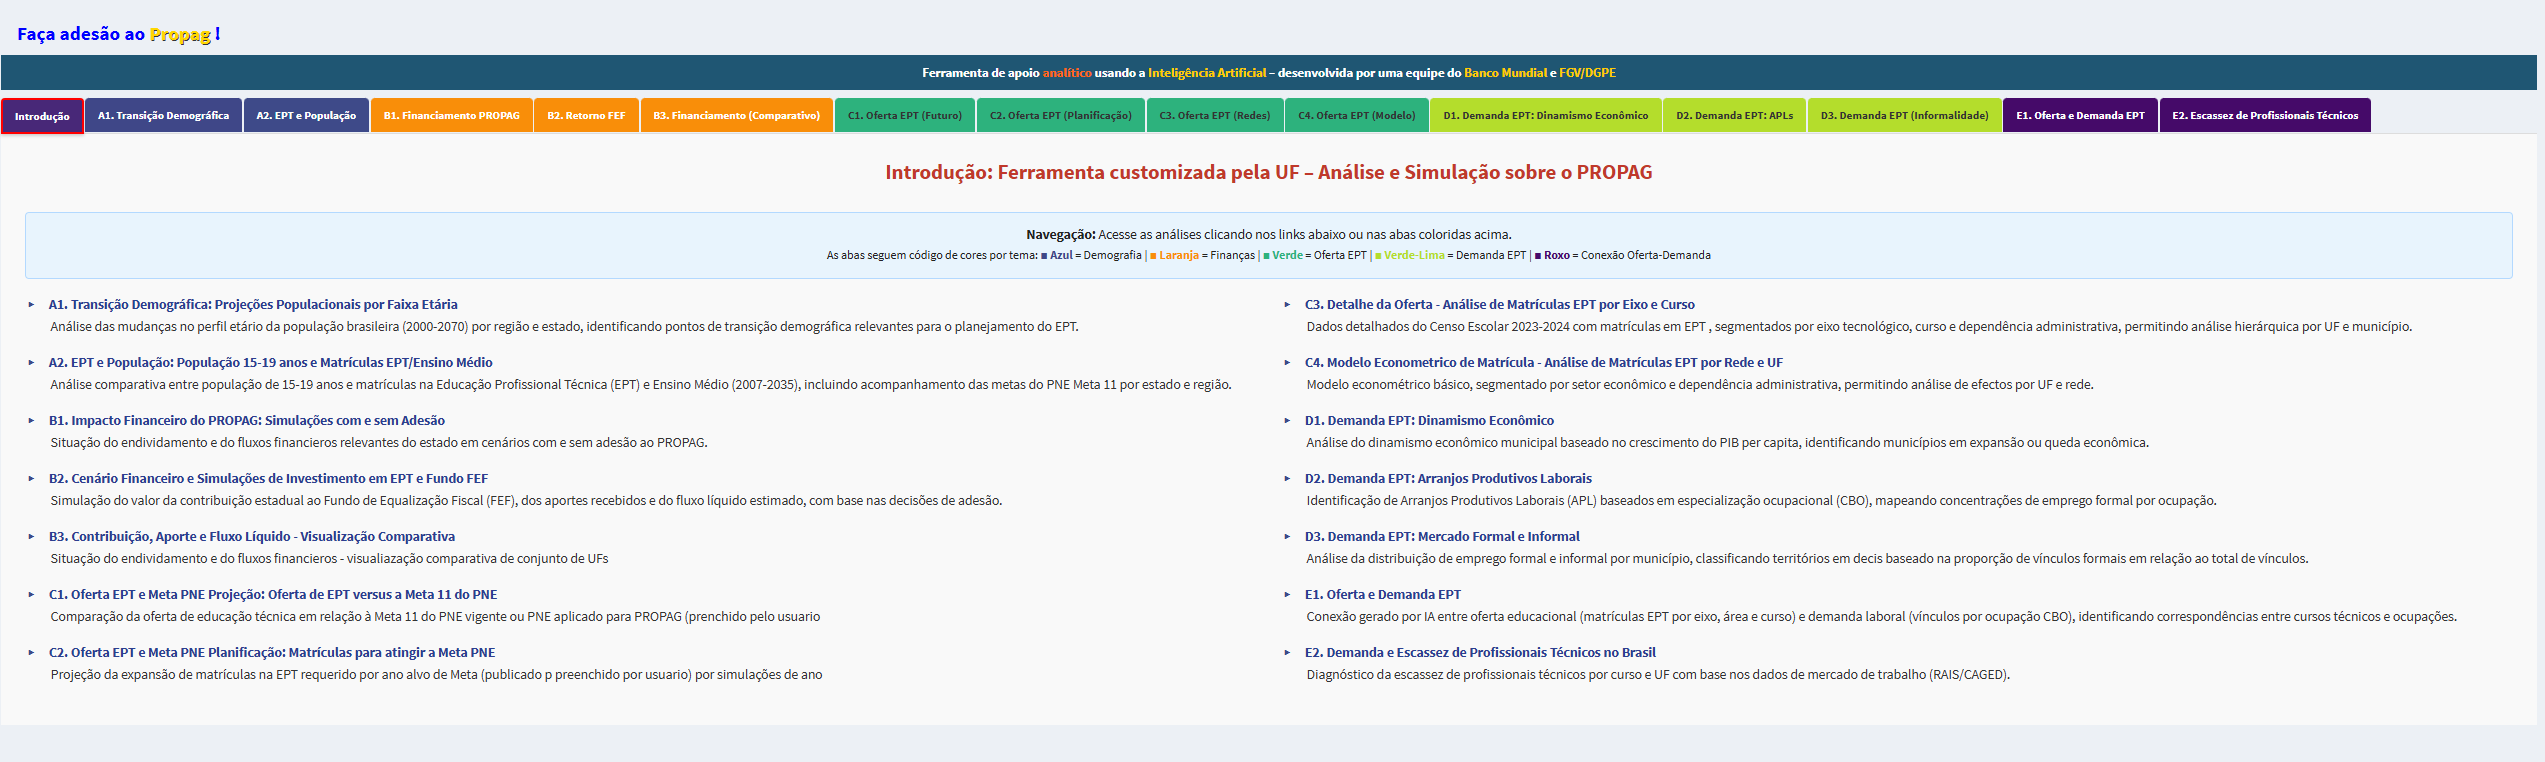
\includegraphics[width=\textwidth]{images/1a_IntroPage.png}
	\caption{Página inicial da Plataforma Analítica Juros por Educação - Interface de navegação com links diretos para todas as análises disponíveis}
	\label{fig:intro_page}
\end{figure}


As análises disponíveis na plataforma incluem:

\begin{itemize}
	\item \textbf{Cenário Financeiro e Simulações:} estima o espaço fiscal gerado pela adesão ao PROPAG e os aportes mínimos em EPT e no Fundo de Equalização Fiscal (FEF).
	
	\item \textbf{Impacto Financeiro com e sem Adesão:} compara a trajetória da dívida estadual em diferentes cenários.
	
	\item \textbf{Retorno do FEF por Opções:} mostra como as escolhas de opção de adesão afetam o saldo líquido estadual.
	
	\item \textbf{Projeções de Oferta e Meta 11 do PNE:} avalia a situação da matrícula em EPT em relação à meta nacional de triplicar o acesso.
	
	\item \textbf{Expansão de Matrículas e Novo PNE (2025--2035):} explora cenários para a próxima década de políticas educacionais.
	
	\item \textbf{Demanda e Escassez de Profissionais Técnicos:} cruza dados do mercado de trabalho (RAIS/CAGED) com a oferta de EPT para mapear gargalos regionais.
\end{itemize}

Além disso, a plataforma inclui \textbf{módulos demográficos} que permitem ao gestor compreender como a dinâmica etária afeta a demanda futura por educação, saúde e serviços sociais.


Com isso, a \textbf{Plataforma Analítica Juros por Educação do BM--FGV} funciona como um verdadeiro \textit{laboratório de simulação e análise}: o administrador estadual pode visualizar a situação do seu estado, comparar cenários de adesão ou não adesão ao PROPAG e planejar a aplicação dos recursos de forma estratégica, alinhando sustentabilidade fiscal, expansão da EPT e enfrentamento dos desafios demográficos.

A partir da página inicial, os usuários podem:
\begin{itemize}
	\item Navegar diretamente para qualquer análise clicando nas abas superiores coloridas
	\item Utilizar os links rápidos na página de introdução para acessar análises específicas
	\item Visualizar a organização temática completa da ferramenta
\end{itemize}

\vspace{1cm}

\clearpage  % for vertical line text


\chapter{População para EPT} \label{ch:popu}
\section{Transição Demográfica} \label{sec:transicao}

O Brasil atravessa uma transição demográfica acelerada: a população de 0–14 anos está em queda contínua, enquanto a de 60 anos ou mais cresce rapidamente, com o ponto de cruzamento previsto por volta de 2029. Esse envelhecimento traz implicações profundas para diferentes dimensões de política pública, inclusive a Educação Profissional e Tecnológica (EPT).


\subsection{Implicações para EPT}

Em primeiro lugar, impõe a necessidade de políticas de requalificação e educação ao longo da vida, já que a força de trabalho será proporcionalmente menor e precisará ser mais produtiva. O crescimento da produtividade no Brasil tem mostrado sinais de estagnação, e esse contexto coloca ainda mais pressão sobre a qualificação dos trabalhadores, tornando a EPT um instrumento essencial para sustentar o desenvolvimento econômico.

\begin{figure}[htbp!]
	\centering
	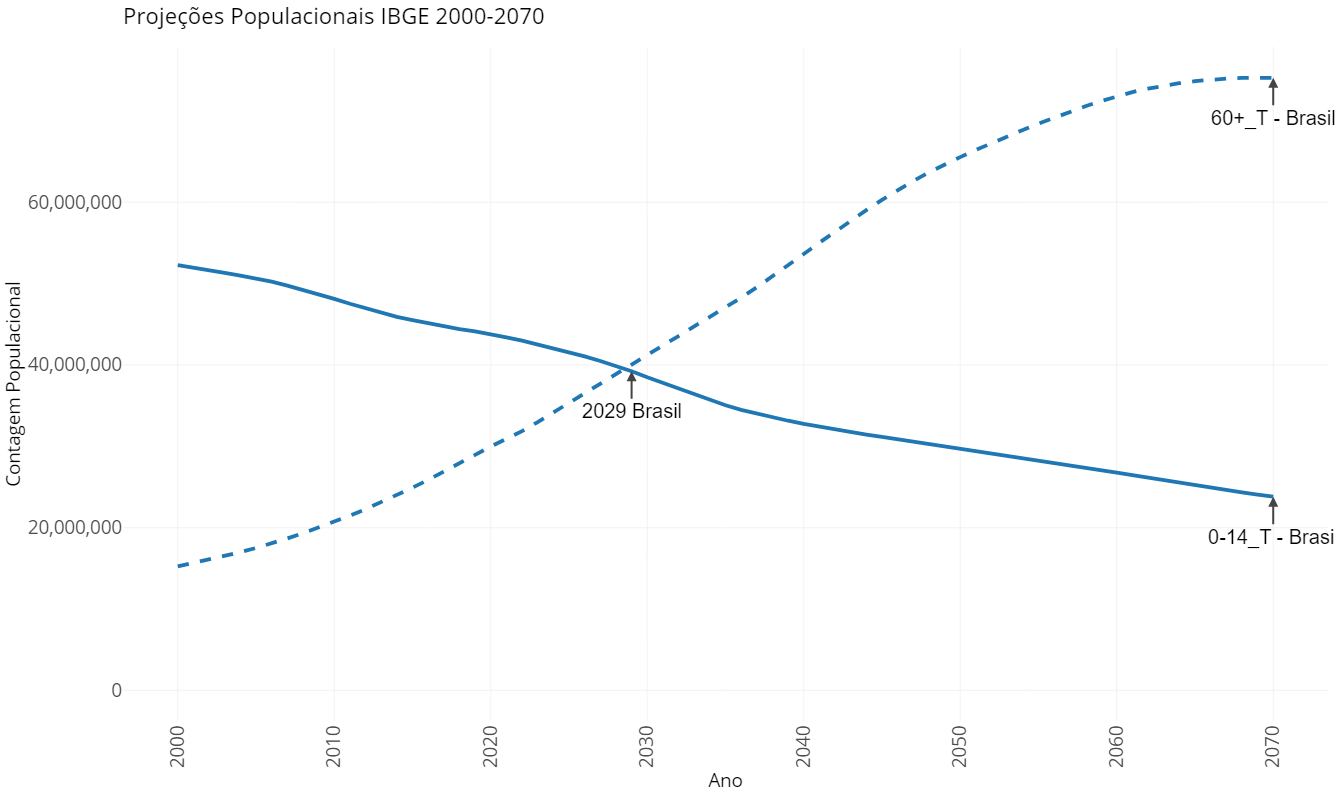
\includegraphics[width=0.75\textwidth]{images/2a_PopuBra.png}
	\caption{Transição demográfica no Brasil: evolução das populações de 0-14 e 60+ anos (2000-2070)} 
	\label{fig:2a_PopuBra}
\end{figure}

Em segundo lugar, o envelhecimento populacional impacta diretamente a demanda por serviços sociais, sobretudo saúde, cuidados de longa duração e apoio ao idoso. Isso cria tanto oportunidades quanto necessidades de formação em ocupações ligadas a serviços de cuidado, assistência e saúde. Ao mesmo tempo, avanços médicos e hábitos de vida mais saudáveis permitem que pessoas idosas permaneçam ativas por mais tempo, o que reforça a importância da requalificação e do reingresso no mercado de trabalho para essa faixa etária.

Por fim, é importante notar que essa transição não ocorre de forma homogênea no território brasileiro: estados com população jovem por mais tempo enfrentam o desafio imediato de expandir a oferta de EPT para absorver grandes coortes de jovens, enquanto estados já envelhecidos precisam ajustar suas estratégias para equilibrar a formação inicial com programas de requalificação e atualização contínua.

\subsection{Implicações para EPT}





\begin{itemize}
\item{pellentesque habitant morbi tristique}
\item{senectus et netus et malesuada fames ac turpis egestas}
\item{ut sit amet ultricies nisl}
\item{etiam laoreet condimentum lacus et elementum}
\end{itemize}

Sed vehicula quis ligula non fermentum. Pellentesque semper ligula gravida "$C_i$",
bibendum dui ut, semper nibh. Quisque a risus porta, fermentum velit vitae,
pellentesque felis.


\begin{figure}[hb]
	\centering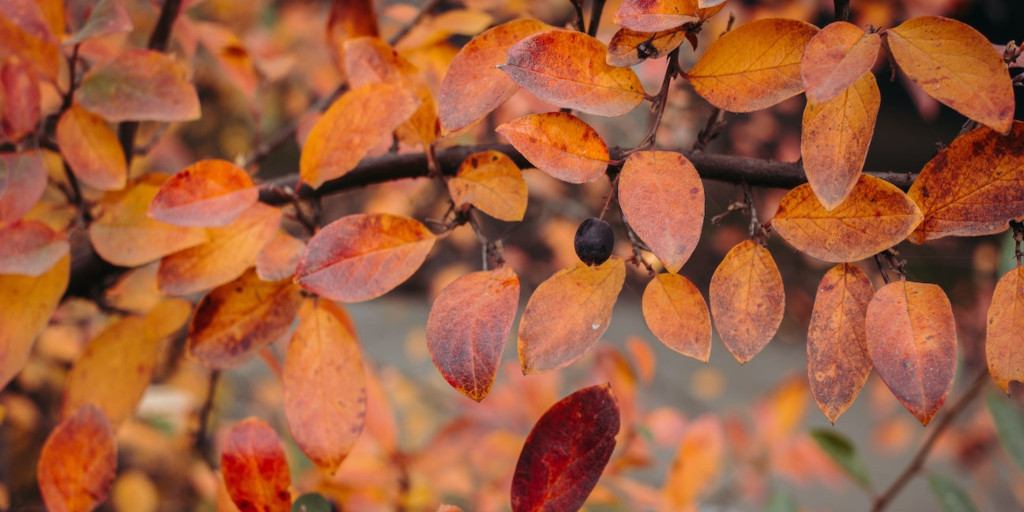
\includegraphics[scale=1]{images/orange2.jpg}
	\caption{Maecenas varius orci vitae eros euismod placerat} \label{fig:integer}
\end{figure}



\newpage
\subsection{Phasellus et quam}

Suspendisse potenti. Aliquam id metus in purus imperdiet aliquam eu ut dolor :

\begin{highlight}
\begin{align}
\alpha_{i+1} &= \frac{A_{i+1}}{S_{i+1}} \\
             &= \frac{A_i + \Delta A_i}{S_i + \Delta S_i} \\
             &= \frac{A_i + \Delta A_i}{S_i + \frac{\Delta A_i}{\alpha_i}} \\
             &= \alpha_i * \frac{A_i + \Delta A_i}{\alpha_i * S_i + \Delta A_i} \\
             &= \alpha_i
\end{align}
\end{highlight}

Vestibulum luctus consectetur vestibulum. Duis ullamcorper ligula nec mauris
viverra rhoncus. Aliquam auctor est accumsan odio vehicula ornare.

\begin{remark}
Duis et metus auctor, fringilla nulla non, dapibus felis \ref{sec:proin}.
\end{remark}

Morbi ipsum dui, rutrum et cursus a, porta eu ligula. Nulla lobortis leo eget
odio bibendum rhoncus. Maecenas posuere nulla nec felis viverra blandit.

\subsection{Felis nunc}

Sit amet elementum tortor malesuada quis. Quisque pellentesque nisl quis augue
interdum vehicula. Nunc nec dictum sem. Nunc venenatis elementum hendrerit \href{https://example.com/}{example.com}.

\begin{remark}
Pellentesque ut justo arcu. Fusce cursus luctus tortor eu venenatis.
\end{remark}

Maecenas viverra dui vitae eros tristique, porta elementum mi aliquam. Cras
sodales erat et molestie auctor. Phasellus mauris eros, bibendum sit amet
rhoncus id, bibendum ut velit.


\newpage
\thispagestyle{empty}
%\mbox{}

-------------------------------------------------
\newpage
\chapter{Cenários de Financiamento no PROPAG}\label{ch:cen_fin}
\section{Cenários Financieros}



\section{Introdução e Contexto}

O Programa de Pleno Pagamento das Dívidas dos Estados – PROPAG, instituído por meio da Lei Complementar n º 212 de 13 de janeiro de 2025, foi concebido como uma forma estratégica de oportunizar a recuperação e o equilíbrio fiscal dos estados, com a possibilidade da revisão dos termos das dívidas que estes possuem com a União, priorizando investimentos em áreas prioritárias, de grande interesse social.

No âmbito do Propag, por meio do Decreto nº 12.433 de 14 de abril de 2025, foi instituído do programa Juros por Educação, que tem como objetivo principal, priorizar investimentos em educação profissional de tecnológica de nível médio (EPTNM).

Este programa determina que, no mínimo, 60\% (sessenta por cento) dos recursos provenientes dos juros não pagos à união e dos oriundos do Fundo de Equalização Federativa (FEF), sejam investidos em iniciativas que promovam a expansão, a manutenção e o fortalecimento da educação profissional e tecnológica em nível médio nos estados, objetivando alcançar as metas de anuais de desempenho estabelecidas pelo Plano Nacional de Educação (PNE).

Pensando também em atender aos estados que estão em dia com suas responsabilidades fiscais e que não possuem dívidas com a União, o programa permite que estes estados também possam aderir ao programa e possam participar da distribuição dos recursos que serão aportados Fundo de Equalização Federativa.

Para oportunizar a participação dos estados que não possuem dívidas com a União e, de certa forma, beneficiar estes estados, será criado o Fundo de Equalização Federativa (FEF), onde os estados endividados que optarem por aderir ao Propag, deverão aportar anualmente um percentual do seu saldo devedor para compor esse fundo, o qual será distribuído anualmente entre todos os estados que aderirem ao Propag na proporção determinada pelo art. 46, incisos I e II do Decreto 12.433/2025.

Quanto aos prazos, os estados têm até o dia 31 de dezembro de 2025 para aderirem ao Propag, devendo para tanto, formalizar sua intenção por meio do envio de um ofício do Chefe do Poder Executivo do estado à Secretaria do Tesouro Nacional, indicando sua intenção de aderir ao Propag, a indicação dos ativos que pretende oferecer à União e a indicação de lei autorizativa devidamente publicada no Diário Oficial.

Os estados deverão apresentar Plano de Aplicação dos Recursos, um para o exercício de 2025 e outro para o exercício de 2026, contemplando, no mínimo, a previsão total de matrículas para o ano subsequente, indicativo do quantitativo de matrículas a serem realizadas pela rede estadual e por meio de parcerias, a previsão de cursos e matrículas e suas justificativas de escolha e a estimativa de investimentos complementares para cumprir o mínimo de 60\% (sessenta por cento) em educação profissional e tecnológica de nível médio.

O prazo para apresentar os Planos de Aplicação para 2025 e 2026 é de até 30 dias após a assinatura do Termo de Aditivo pelo estado, ou até 30 de outubro de 2025, o que ocorrer primeiro. Após 30 de outubro de 2025, os estados deverão apresentar o Plano de Aplicação no momento da assinatura do Termo Aditivo. 

Os demais 40\% (quarenta por cento) dos recursos oriundos do Propag, poderão ser investidos em universidades estaduais, infraestrutura educacional, saneamento, habitação, segurança pública e adaptação climática.

Para 2025, as metas a serem alcançadas seguem os parâmetros do PNE vigente (2014 – 2025). Para 2026, caso seja aprovado o novo PNE, as metas deverão ser alteradas para obedecer aos parâmetros deste novo plano.


\section{Projeção das dívidas}

Conforme relatado, a criação do Programa de Pleno Pagamento das Dívidas dos Estados, o PROPAG, tem como objetivo principal, proporcionar aos estados que possuem dívidas com a União, condições de refinanciar e quitar suas dívidas no prazo de 360 meses, com a possibilidade de zerar os juros incidentes sobre o saldo devedor, permitindo o equilíbrio financeiro destes entes, culminando na retomada do crescimento e do desenvolvimento econômico e social.

Com o objetivo de demonstrar as possíveis vantagens financeiras que a adesão ao Propag poderá trazer aos estados, buscou-se apresentar uma simulação da evolução do crescimento das dívidas de alguns estados nos últimos 5 anos (2021 – 2025), bem como, uma simulação da projeção destas dívidas nos próximos 10 anos (2026 – 2035), a qual foi representada em um quadro evolutivo, simulando 3 cenários diferentes, onde estes estados, supostamente, optam primeiro, por não aderir ao programa Propag, num segundo cenário, aderindo e fazendo um abatimento do saldo devedor de 20\% (vinte por cento) e, num  terceiro cenário, optando por aderir sem fazer nenhum abatimento no saldo devedor. 

Seguindo a tabela evolutiva, apresentamos um gráfico comparativo, demonstrando a evolução do saldo devedor em cenários simulados.

Cabe lembrar que, por se tratar de um refinanciamento das dívidas estaduais feitas com base na tabela Price, com correção pelo índice IPCA, pelo prazo de 360 meses, a tendência de redução nos valores das prestações, começa a ser perceptível a partir da metade final do prazo, entre os últimos anos. 


\begin{figure}[htbp!]
	\centering
	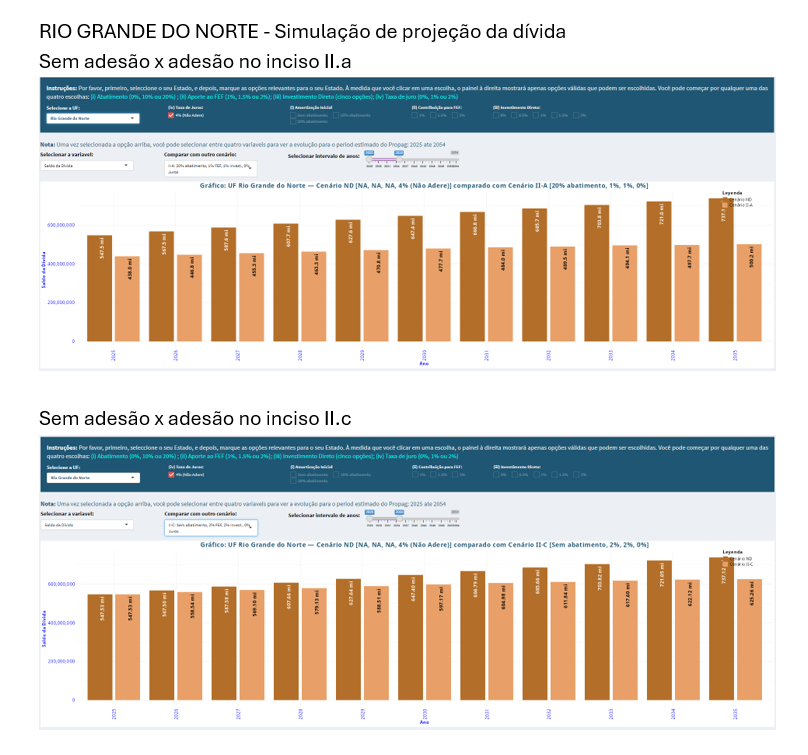
\includegraphics[width=1\textwidth]{images/7a.png}
	\caption{Aba E: Análise de Cenários EPT} 
	\label{fig:7a}
\end{figure}


\begin{figure}[htbp!]
	\centering
	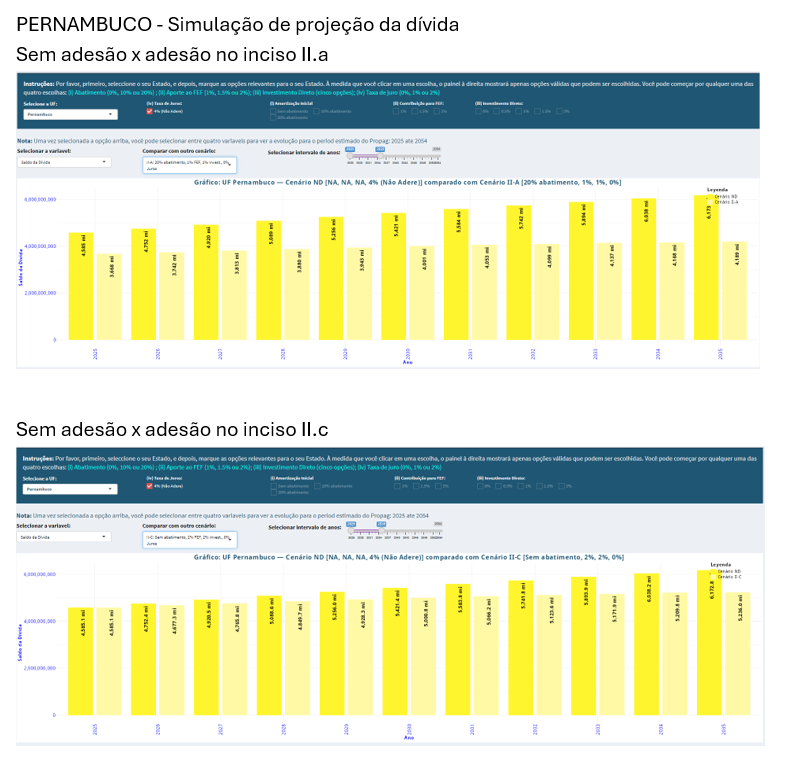
\includegraphics[width=1\textwidth]{images/7b.png}
	\caption{Aba E: Análise de Cenários EPT} 
	\label{fig:7b}
\end{figure}


\begin{figure}[htbp!]
	\centering
	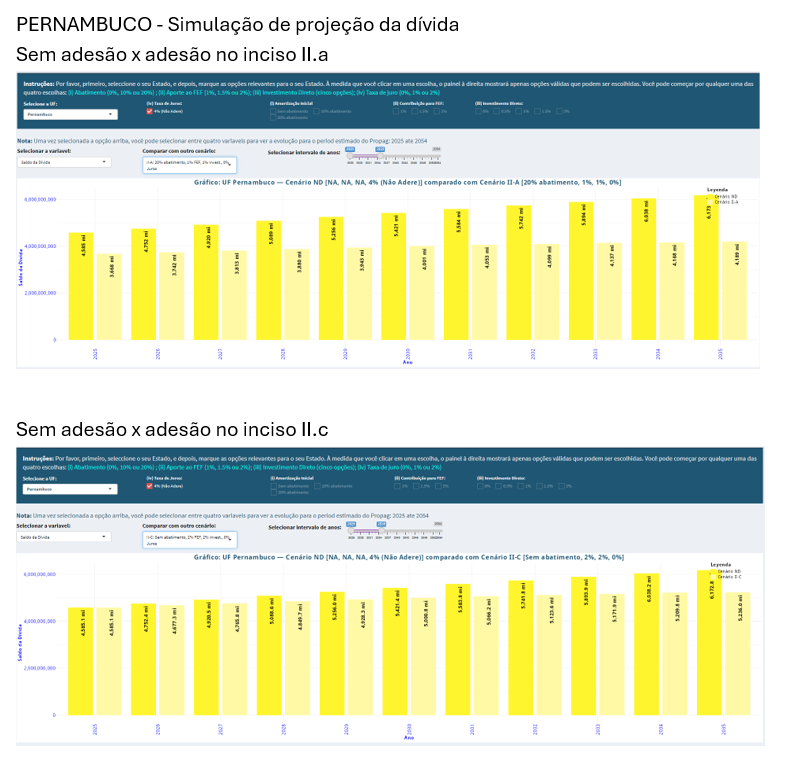
\includegraphics[width=1\textwidth]{images/7b.png}
	\caption{Aba E: Análise de Cenários EPT} 
	\label{fig:7c}
\end{figure}


\section{Opções de adesão}

Os estados que optarem por aderir ao Propag, deverão escolher uma dentre as 8 formas de adesão ao programa.

São 3 opções de taxa de juros que irão incidir sobre o saldo devedor que são de 0\% (zero) no inciso II, 1\% (um por cento) no inciso III e 2\% (dois por cento) no inciso IV. 

Além da escolha da taxa de juros, o estado deverá escolher uma das opções de amortização do saldo devedor, que pode ser de 0\% (zero), 10\% (dez por cento) ou 20\% (vinte por cento) que irão incidir sobre o valor do saldo devedor. Nesta amortização, o estado poderá oferecer ativos à União, como bens móveis e imóveis, créditos, participações societárias, etc., como forma de abatimento.

Cumpre lembrar que, mesmo os estados que não possuem dívidas com a União, poderão aderir ao Propag, e poderão participar da distribuição dos recursos do Fundo de Equalização Federativa, sem a necessidade de contribuir para este fundo.

Conforme a opção do estado, por taxa de juros e percentual de amortização, ele se enquadrará em uma das opções da tabela abaixo no que diz respeito ao percentual de aporte e de investimentos internos diretos:


\begin{figure}[htbp!]
	\centering
	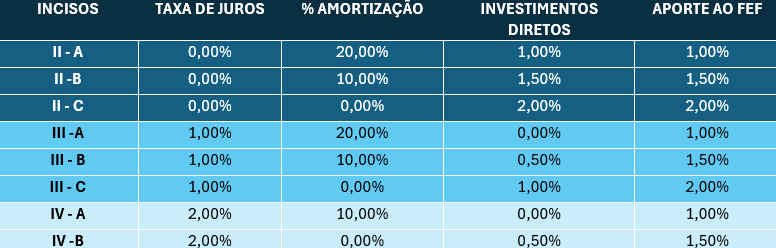
\includegraphics[width=1\textwidth]{images/7_opcoes.png}
	\caption{Aba E: Análise de Cenários EPT - Opções } 
	\label{fig:7_opcoes}
\end{figure}


\subsection{Simulação comparativa das opções de adesão}

Com o objetivo de realizar um comparativo entre duas das oito opções de adesão ao Propag, apresenta-se abaixo, algumas simulações de aporte ao FEF com os estados optando por aderir na opção do inciso II.a, com taxa de juros 0\% e 20\% de amortização do saldo devedor em comparação com a opção de adesão do mesmo estado no inciso II.c, com taxa de juros 0\% e amortização de 0\% sobre o saldo devedor.


\begin{figure}[htbp!]
	\centering
	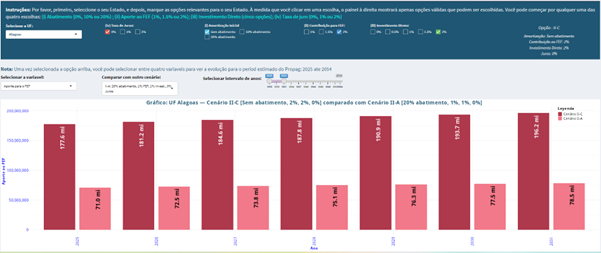
\includegraphics[width=1\textwidth]{images/7f.png}
	\caption{Simulação de Aporte ao FEF - Alagoas: Opção II.a x Opção II.c} 
	\label{fig:7f}
\end{figure}

\begin{figure}[htbp!]
	\centering
	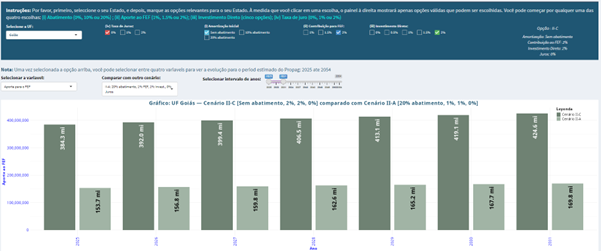
\includegraphics[width=1\textwidth]{images/7g.png}
	\caption{Simulação de Aporte ao FEF - Goiás: Opção II.a x Opção II.c} 
	\label{fig:7g}
\end{figure}

\begin{figure}[htbp!]
	\centering
	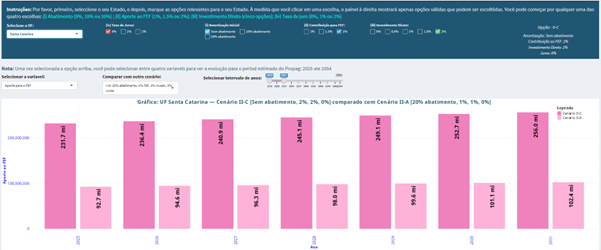
\includegraphics[width=1\textwidth]{images/7h.png}
	\caption{Simulação de Aporte ao FEF - [Estado]: Opção II.a x Opção II.c} 
	\label{fig:7h}
\end{figure}


\section{Simulação de retorno do FEF}

O Fundo de Equalização Federativa (FEF), é formado pelo aporte anual de percentual do saldo devedor dos estados que aderirem ao programa Propag, conforme as opções apresentadas anteriormente.

Após realizado o aporte pelos entes participantes, o valor resultante é dividido entre todos os estados que aderirem ao Propag, independentemente de ter ou não saldo devedor com a União.

O percentual de participação de cada estado é determinado pelo art. 46, incisos I e II do Decreto 12.433/2025, que estipula que a remuneração terá como critérios, o inverso da relação entre a Dívida Consolidada e a Receita Corrente Líquida com peso de 20\%, e o coeficiente de participação no Fundo de Participação dos Estados, com peso de 80\%.

A seguir, optou-se por representar um gráfico com uma simulação do valor devido para alguns estados, com 3 cenários diversos, conforme segue:

\begin{enumerate}
	\item Uma projeção simulada com a participação de todos os estados aderindo ao Propag pelo inciso II.a, com juros 0\% e amortização do saldo devedor de 20\%.
	\item Uma projeção simulada com a participação de todos os estados aderindo ao Propag, pelo inciso II.b, com juros 0\% e amortização do saldo devedor de 10\%.
	\item Uma projeção simulada com a participação de todos os estados aderindo ao Propag, pelo inciso II.c, com juros 0\% e amortização do saldo devedor de 0\%.
\end{enumerate}

\begin{figure}[htbp!]
	\centering
	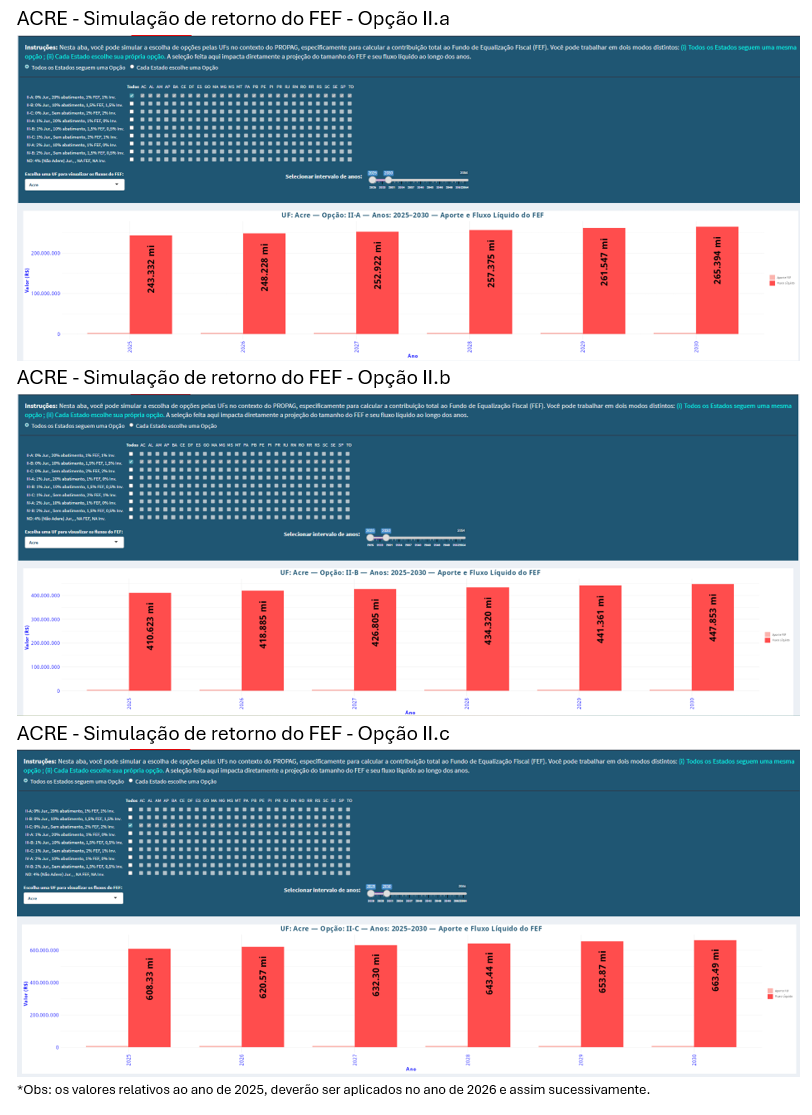
\includegraphics[width=1\textwidth]{images/7m.png}
	\caption{Simulação de Retorno do FEF - Acre: Comparação das Opções II.a, II.b e II.c} 
	\label{fig:7m}
\end{figure}


\begin{figure}[htbp!]
	\centering
	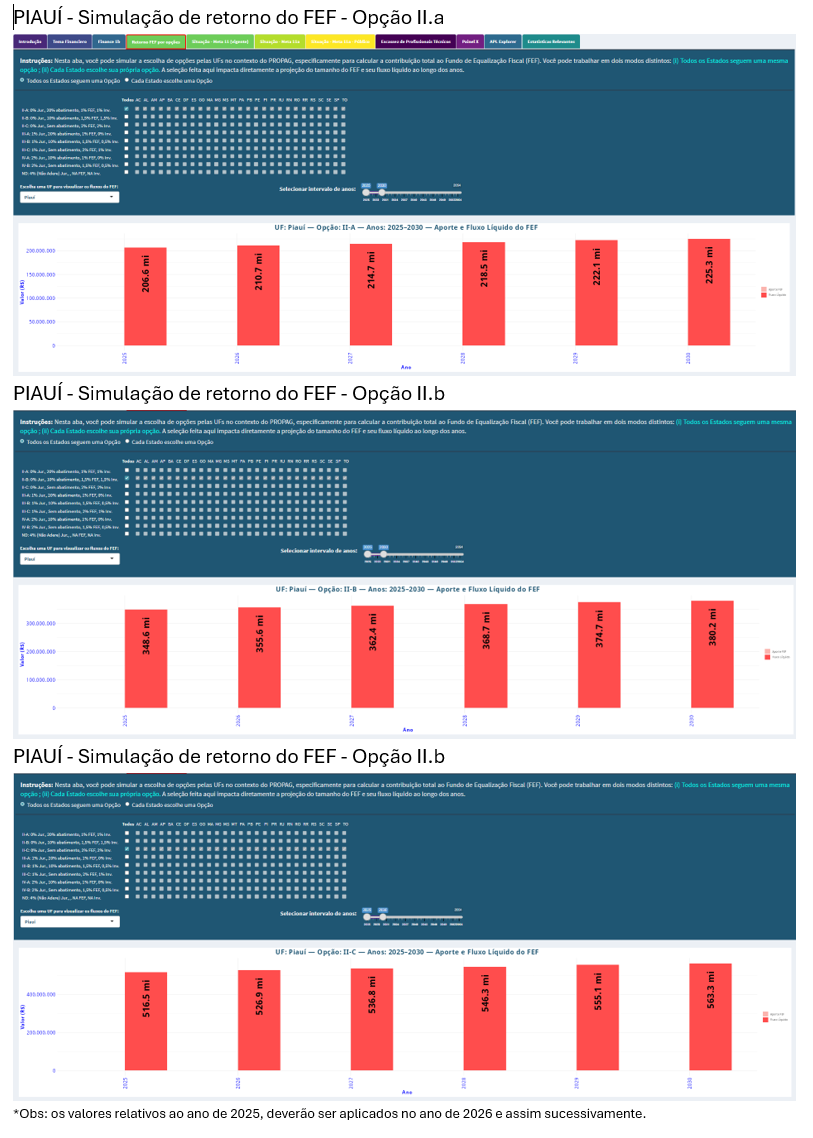
\includegraphics[width=1\textwidth]{images/7n.png}
	\caption{Simulação de Retorno do FEF - Piauí: Comparação das Opções II.a, II.b e II.c} 
	\label{fig:7n}
\end{figure}
\clearpage

\newpage
\thispagestyle{empty}
\mbox{}

\part{Oferta e Demanda de \hspace{-1em} EPT}

\newpage
\thispagestyle{empty}
\mbox{}


\chapter{Oferta de EPT e Meta PNE} \label{ch:metas_pne}
\section{PNE Vigente} 

\subsection{Metas estabelecidas}

No Plano Nacional de Educação (2014-2024), a Meta 11 estabelecia o objetivo de triplicar as matrículas da Educação Profissional Técnica de Nível Médio (EPTNM) até 2024, assegurando que pelo menos 50\% da expansão ocorresse na rede pública. A tabela a seguir apresenta:
\begin{itemize}
	\item A meta definida para cada estado no PNE vigente;
	\item O total de matrículas de EPTNM registrado no Censo Escolar 2024;
	\item O déficit em relação à meta, a ser considerado para a elaboração do Plano de Aplicação de Recursos.
\end{itemize}

As matrículas de todas as redes de ensino foram consideradas nos dados a seguir. 

\begin{table}[!htbp] \centering 
	\caption{Meta 11 do PNE vs Matrículas Efetivas em EPTNM por Estado}
	\label{tab:meta11deficit}
	\footnotesize
	\begin{tabular}{@{\extracolsep{5pt}} lrrr} 
		\\[-1.8ex]\hline 
		\hline \\[-1.8ex] 
		Brasil e Estados & Meta 11 do PNE & Total de Matrículas de & Déficit de matrículas em \\
		& Matrículas em EPTNM & EPTNM (Censo, 2024) & relação à meta 11 \\ 
		\hline \\[-1.8ex] 
		Brasil & 4.614.621 & 2.352.083 & 2.262.538 \\ 
		Acre & 6.652 & 8.492 & - \\ 
		Alagoas & 42.507 & 24.589 & 17.918 \\ 
		Amapá & 15.903 & 5.605 & 10.298 \\ 
		Amazonas & 66.552 & 44.127 & 22.425 \\ 
		Bahia & 265.644 & 177.727 & 87.917 \\ 
		Ceará & 156.246 & 114.569 & 41.677 \\ 
		Distrito Federal & 45.342 & 30.053 & 15.289 \\ 
		Espírito Santo & 144.543 & 60.568 & 83.885 \\ 
		Goiás & 80.087 & 37.664 & 42.423 \\ 
		Maranhão & 76.029 & 71.075 & 4.924 \\ 
		Mato Grosso & 61.326 & 21.040 & 40.286 \\ 
		Mato Grosso do Sul & 61.821 & 20.928 & 40.893 \\ 
		Minas Gerais & 535.443 & 259.015 & 276.428 \\ 
		Pará & 77.283 & 61.194 & 16.089 \\ 
		Paraíba & 47.346 & 52.368 & - \\ 
		Paraná & 321.561 & 158.011 & 163.550 \\ 
		Pernambuco & 189.324 & 108.228 & 81.096 \\ 
		Piauí & 82.350 & 99.338 & - \\ 
		Rio de Janeiro & 489.018 & 146.789 & 342.229 \\ 
		Rio Grande do Norte & 69.348 & 55.628 & 13.720 \\ 
		Rio Grande do Sul & 314.736 & 138.757 & 175.979 \\ 
		Rondônia & 26.256 & 11.583 & 14.673 \\ 
		Roraima & 12.000 & 4.045 & 7.955 \\ 
		Santa Catarina & 197.310 & 82.602 & 114.708 \\ 
		São Paulo & 1.184.199 & 531.906 & 652.893 \\ 
		Sergipe & 13.386 & 15.532 & - \\ 
		Tocantins & 31.959 & 10.500 & 21.459 \\ 
		\hline \\[-1.8ex] 
	\end{tabular} 
\end{table}

No \textbf{Painel C1: PNE Vigente}, o gestor pode selecionar seu estado e visualizar a projeção do Ensino Médio e da EPTNM até 2035. Esse módulo foi desenhado para apoiar tecnicamente o desenvolvimento do Plano de Aplicação de Recursos pelos estados aderentes ao PROPAG, evidenciando a distância em relação à meta nacional e os desafios específicos de expansão. Além da opção de utilizar a Meta 11 estabelecida no PNE (2014–2024), o usuário também pode definir um valor alternativo de meta, de acordo com eventuais anúncios do MEC sobre os números oficiais de referência da Meta 11 para cada unidade da federação, que serão adotados no âmbito do PROPAG.



\begin{figure}[htbp!]
	\centering
	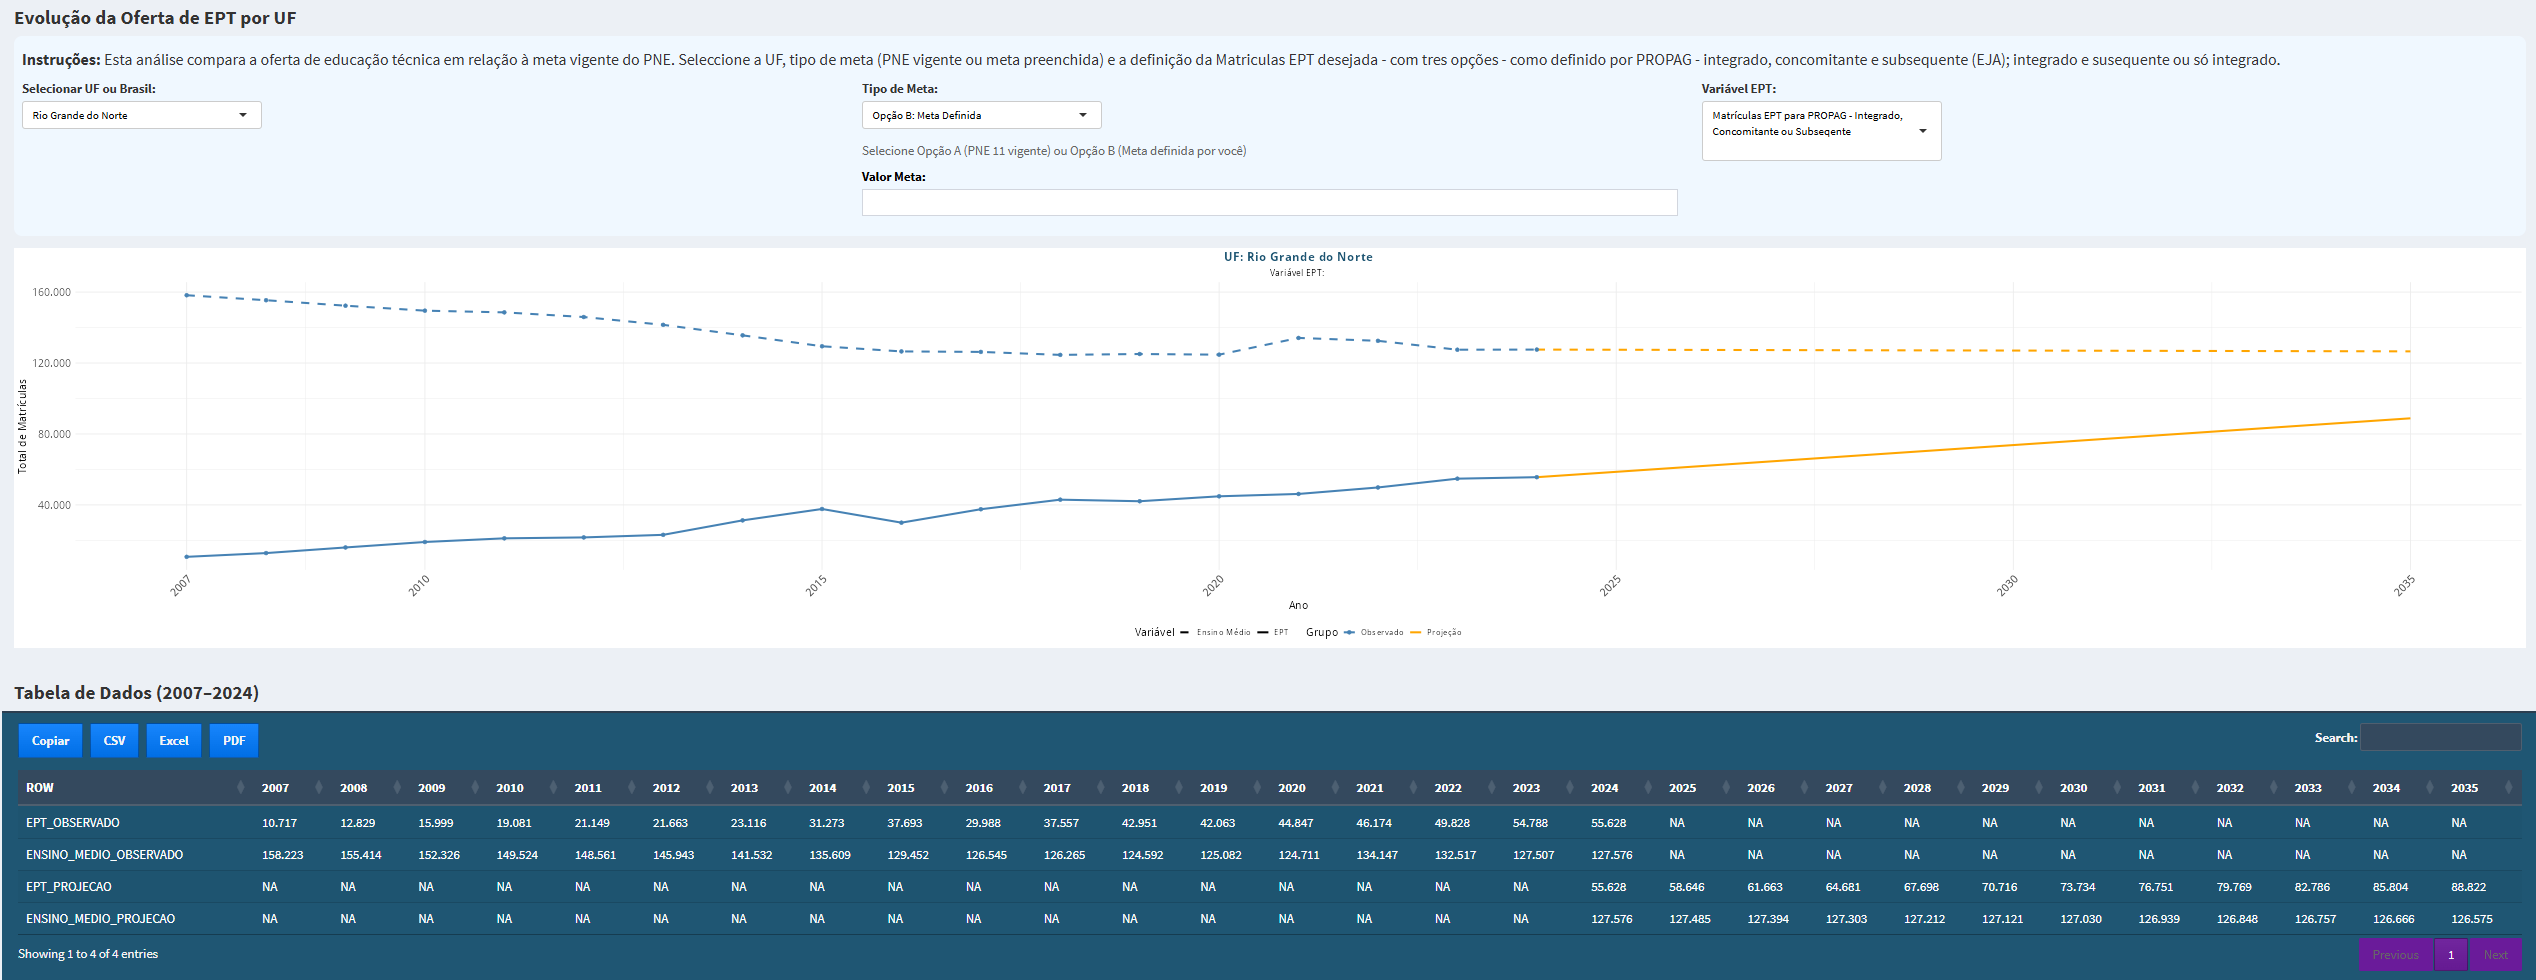
\includegraphics[width=1\textwidth]{images/TabC1_1a.png}
	\caption{Painel C1: Evolução da Oferta em relação à Meta 11 do PNE} 
	\label{fig:6a_Meta11}
\end{figure}

\subsection{Expansão das matrículas em EPT 2014-2024} 

Com base nos dados da Meta 11 do PNE, observa-se que o Brasil ainda está distante de alcançar a meta de 4,6 milhões de matrículas em EPTNM, registrando atualmente 2,35 milhões, com um déficit de 2,26 milhões de vagas. Estados populosos como São Paulo, Rio de Janeiro e Minas Gerais concentram a maior parte desse déficit, enquanto estados como Acre, Paraíba, Piauí e Sergipe já superaram a meta, indicando boas práticas locais que podem servir de referência. Há uma clara desigualdade regional: o Sudeste acumula o maior déficit absoluto, o Centro-Oeste apresenta lacunas proporcionais significativas, e o Nordeste mostra resultados mistos. 

Para atingir a meta, será necessário um crescimento acelerado e estratégico, priorizando estados com maior déficit absoluto e proporcional, ao mesmo tempo em que se aproveitam experiências bem-sucedidas em regiões que já superaram a meta. Essa constatação conduz diretamente à análise prospectiva apresentada no \textbf{Painel C2}, que permite comparar diferentes definições da Meta 11a, selecionar o ano-alvo para o seu cumprimento e calcular o incremento anual necessário de matrículas em cada cenário.


\section{PNE (2025–2035) na discussão}

\subsection{Política de Expansão da EPT}

Com a proximidade do encerramento do PNE 2014–2024 e a tramitação do novo PNE (2025–2035), o debate sobre a política de expansão da Educação Profissional Técnica de Nível Médio (EPTNM) torna-se central. O \textbf{Painel C2} foi desenvolvido para apoiar esse processo, permitindo que os gestores estaduais comparem diferentes definições da Meta 11a, selecionem o ano-alvo para o seu cumprimento e calculem o incremento anual necessário de matrículas em cada cenário.

A tabela a seguir organiza os principais elementos de análise:
\begin{itemize}
	\item O cenário atual das matrículas em EPTNM (Censo 2024);
	\item A projeção de matrículas no Ensino Médio em 2035;
	\item O aumento anual necessário de estudantes para atingir a meta;
	\item O percentual adicional de crescimento por ano até o ano-alvo.
\end{itemize}

Por fim, o painel contempla todas as redes de ensino e considera a EPTNM nas modalidades integrado, concomitante, subsequente e EJA, em conformidade com o escopo estabelecido para o PROPAG. O usuário pode ainda ajustar o crescimento projetado do Ensino Médio e simular diferentes horizontes de expansão, conforme a definição da meta utilizada pelo MEC ou valores alternativos adotados para o plano estadual.

\begin{figure}[htbp!]
	\centering
	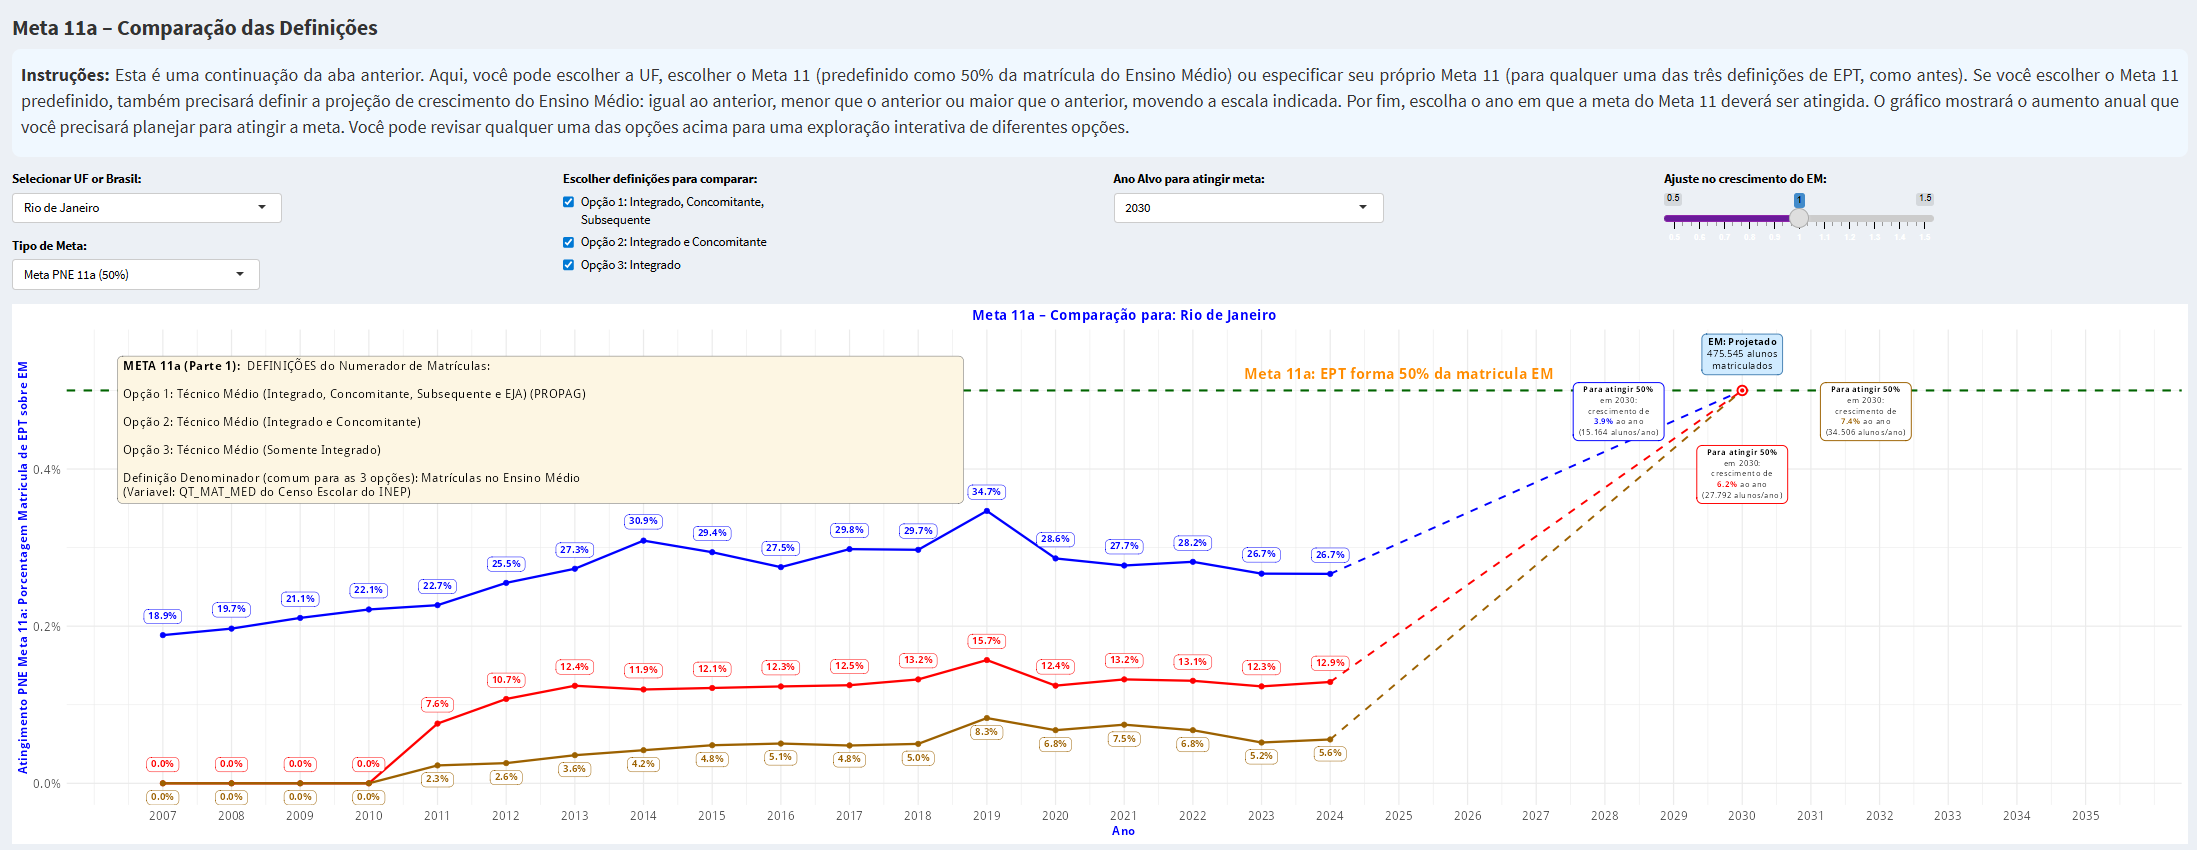
\includegraphics[width=1\textwidth]{images/TabC2_1a.png}
	\caption{Painel C2: Comparação das Definições da Meta 11a e Ano-Alvo}
	\label{fig:6b_Meta11a}
\end{figure}

\subsection{Trajetórias e Incrementos Necessários}

O Painel C2 mostra de forma interativa que a trajetória para o alcance da meta depende tanto da definição adotada para o numerador (todas as modalidades, apenas integrado e concomitante, ou apenas integrado) quanto do ano-alvo selecionado. Dessa forma, um estado pode planejar o ritmo de expansão em termos operacionais, expresso em \textit{novas matrículas por ano}, o que facilita a tradução da meta nacional em planos de ação estaduais.

Esse módulo complementa o diagnóstico do Painel C1: enquanto aquele evidencia o déficit atual frente à meta vigente, o Painel C2 oferece as alternativas de expansão para o próximo ciclo decenal de planejamento educacional, transformando o déficit em metas anuais concretas que podem ser incorporadas ao Plano de Aplicação de Recursos.


\section{Ampliação dos recursos para as redes}

Atingir os níveis de expansão projetados no \textbf{Painel C2} exige não apenas planejamento pedagógico, mas sobretudo capacidade financeira. A legislação do PROPAG estabelece que, até o cumprimento da Meta 11 do PNE, pelo menos 60\% dos recursos economizados com juros deverão ser aplicados em EPTNM. Isso significa que a sustentabilidade da trajetória até 2035 dependerá da articulação entre os investimentos constitucionais já realizados pelos estados, as transferências do Novo FUNDEB e os programas federais complementares.

As fontes de financiamento são essenciais para toda política pública, especialmente em um país com a complexidade geográfica, política, social e econômica como a do Brasil. A Educação Profissional precisa de recursos suficientes e estáveis, pois se trata de um processo contínuo, sustentado por professores, pesquisadores, estudantes e profissionais da educação em milhares de escolas distribuídas pelo território nacional.

A adesão ao PROPAG amplia os recursos disponíveis para todos os estados. Ao articular os valores obrigatórios de manutenção e desenvolvimento do ensino com os novos fatores de ponderação do FUNDEB e com programas federais como a Escola em Tempo Integral, os gestores estaduais poderão potencializar a capacidade de expansão e qualificação da oferta de EPT.

\subsection{Implicações do Novo FUNDEB}

Os novos Fatores de Ponderação nos Recursos do FUNDEB orientam a distribuição proporcional dos recursos, multiplicando o número de matrículas por coeficientes diferenciados. As modalidades da Formação Técnica Profissional (FTP) estão entre as mais valorizadas: 1,30 para o ensino médio articulado à educação profissional (curso técnico integrado), 1,40 para o ensino médio integral e 1,20 para a EJA integrada à educação profissional de nível médio. 

A Resolução nº 4, de 30 de outubro de 2023, especificou as diferenças e ponderações para o exercício de 2024, conforme a tabela abaixo:

\newenvironment{nomenclature}[1]
{
	\begin{table}[hbt]
		\caption{#1}
		\begin{center}
			\begin{tabular}{|l|l|l|}
				\hline
				\textbf{Symbol} & \textbf{Unit} & \textbf{Description}\\
				\hline
			}
			{
				\\\hline
			\end{tabular}
		\end{center}
	\end{table}
}

\begin{nomenclature}{Fatores de Ponderação FUNDEB - Resolução nº 4/2023}
	Ensino Médio Integral & 1,40 & um inteiro e quarenta centésimos\\
	Ensino Médio Articulado & 1,30 & um inteiro e trinta centésimos\\
	EJA Integrada EPT & 1,20 & um inteiro e vinte centésimos\\
	Formação Técnica & 1,30 & um inteiro e trinta centésimos
\end{nomenclature}

\subsection{Escola de Tempo Integral}

O Programa Escola em Tempo Integral, instituído pela Lei nº 14.640 de 2023, prevê a criação e ampliação de matrículas em tempo integral em todas as etapas e modalidades da educação básica. O programa assegura assistência técnica e financeira para matrículas com jornada mínima de sete horas diárias ou 35 horas semanais em dois turnos, priorizando estudantes em maior vulnerabilidade socioeconômica. 

As redes estaduais podem articular esse programa diretamente com a expansão da EPT, especialmente na modalidade do Ensino Médio Integrado com Curso Técnico (EMI) ou mesmo no formato concomitante em turnos complementares. Dessa forma, os recursos adicionais do programa não apenas aumentam o tempo de permanência escolar, mas também criam condições estruturais para ampliar a oferta de vagas técnicas em alinhamento com a Meta 11 do PNE.

\bigskip

Em síntese, os instrumentos financeiros — PROPAG, FUNDEB e Escola em Tempo Integral — constituem a base para transformar as trajetórias projetadas no Painel C2 em políticas exequíveis. A articulação entre esses mecanismos será decisiva para que cada unidade da federação consiga sustentar o crescimento anual de matrículas e reduzir as desigualdades regionais de acesso à EPT.


\newpage
\thispagestyle{empty}
\mbox{}


\chapter{Oferta de EPT - Redes e Cursos} 
\section{Panorama Atual sobre EPT no Brasil} 


Neste capítulo apresentamos um panorama nacional sobre as matrículas por tipos de dependência Estadual, Federal, Municipal e Privada (incluído o Sistema S).  Fica evidenciado que o Brasil possui quatro redes robustas que lideram as ofertas, variando sua participação dependendo de cada Estado. No simulador interativo na internet é possível acessar e pesquisar por  UF:
\href{https://datanalytics.worldbank.org/content/6604f317-d487-436a-b6b6-792369b341f0}{https://datanalytics.worldbank.org/Plataforma Interativo PROPAG}  



\begin{figure}[htbp!]
	\centering
	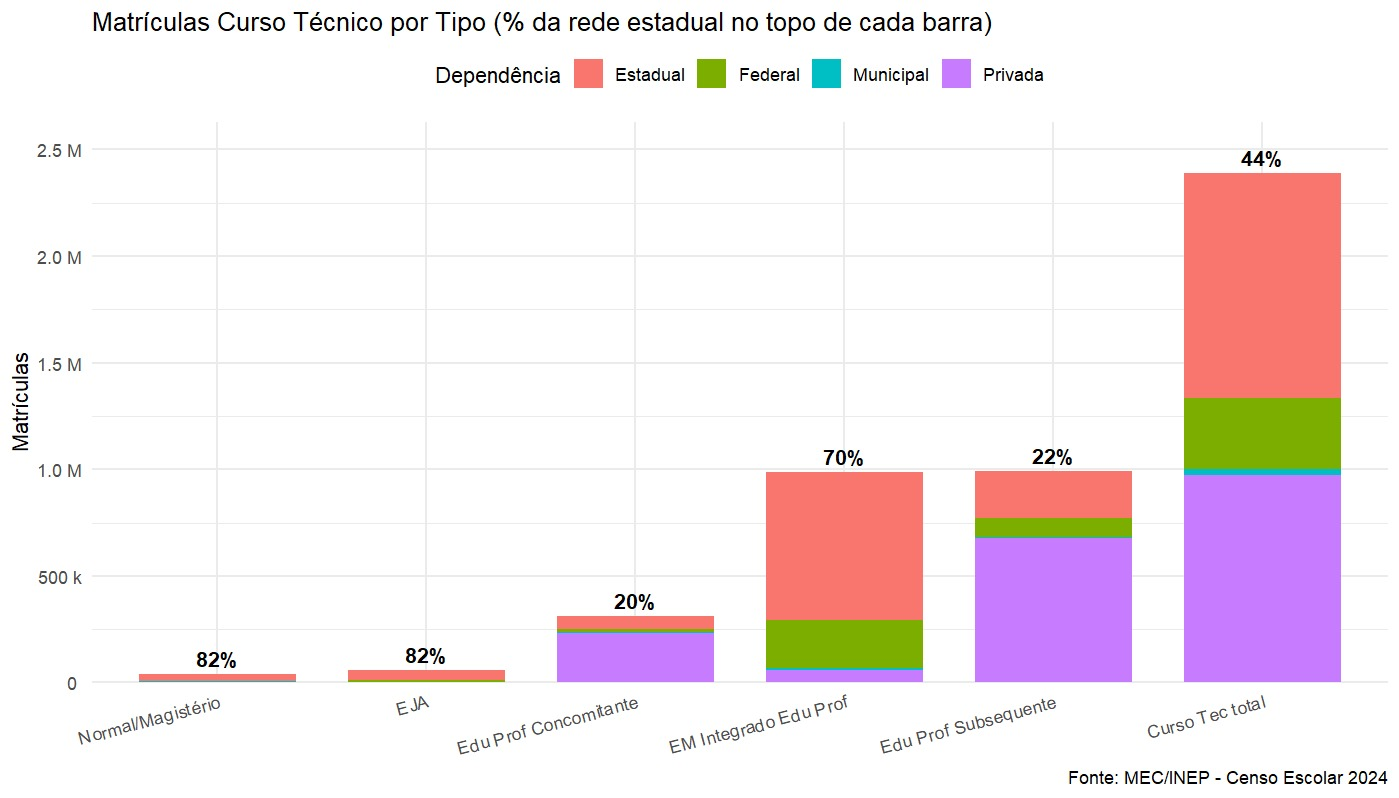
\includegraphics[width=1\textwidth]{images/3a_MaTec.png}
	\caption{Aba C: Matricula Técnicas por tipo} 
	\label{fig:3a_MaTec}
\end{figure}


Este  primeiro gráfico \ref{fig:3a_MaTec} apresenta o cenário da oferta da EPT por meio das diversas redes de ensino. As redes estaduais são as maiores ofertantes, seguidas pela oferta da rede privada (incluindo o Sistema S) e indicam uma evolução da Rede Federal com a expansão dos Institutos Federais (IFs).

O próximo gráfico  \ref{fig:3b_MaTec} na sequência apresenta uma panorâmica das Matrículas de Educação Profissional Técnica (EPT) por Unidade da Federação e a participação de cada rede. Novamente as redes estaduais e a rede privada, com variáveis por UF, lideram também o [\textcolor{red}{MARINA ou TEXTO ACABOU}]

\begin{figure}[htbp!]
	\centering
	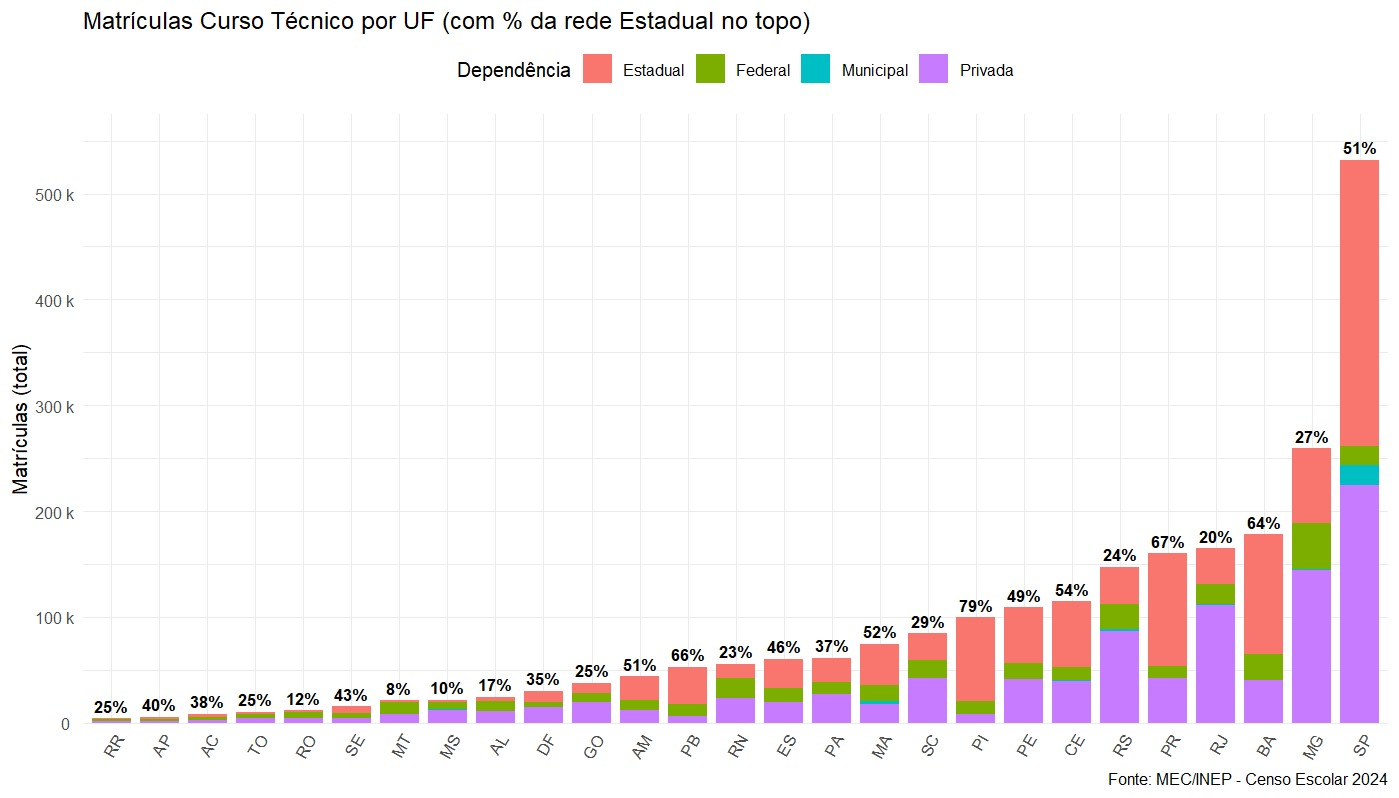
\includegraphics[width=1\textwidth]{images/3b_MaTec.png}
	\caption{Aba C: Matriculas em Curso Técnico por tipo} 
	\label{fig:3b_MaTec}
\end{figure}


\section{Política de coordenação entre redes}

Um dos desafios importantes do Programa de Expansão da EPT no Brasil e nas UFs é a coordenação e articulação das diversas redes e instituições de ensino ofertantes de cursos técnicos. É fundamental a elaboração e consolidação de uma Política Estadual de EPT em cada UF e que sejam superadas as descontinuidades de políticas, programas e projetos após cada ciclo de governo, tanto no âmbito federal como estadual. 

A EPT no Brasil já conta com uma estrutura instalada de instituições públicas e privadas de grande impacto. O país tem 29.993 escolas de ensino médio funcionando; 661 unidades (campi) vinculadas a 38 Institutos Federais (IFs), 02 Centros Federais de Educação Tecnológica (Cefet), uma Universidade Tecnológica Federal do Paraná (UTFPR), 22 escolas técnicas vinculadas às universidades federais e o Colégio Pedro II no Rio de Janeiro, além de ofertas de cursos técnicos em municípios brasileiros.

Como parceiros que já ofertam cerca de 21\% das matrículas de EPT no Brasil destacam-se as Escolas Privadas e Confessionais; o Sistema S, nome do conjunto das organizações criadas pelos setores produtivos (indústria, comércio, agricultura, transportes, cooperativas e microempresas), voltadas para qualificação profissional, pesquisa e assistências técnica e social com mais de 500 escolas em 3.431 unidades e, ainda, 2.264 Instituições Privadas de Ensino Superior (IPES).

O PROPAG apresenta uma oportunidade na perspectiva de  priorização e potencialização de todas as estruturas das diversas redes e parceiros para focar os investimentos na ampliação das matrículas e nas condições de ensino-aprendizagem dos estudantes da EPT. É uma oportunidade histórica para cada Estado e para o país formação de uma grande geração de técnicos de nível médio antes da transição demográfica estrutural em curso.

\newpage
\thispagestyle{empty}
\mbox{}

\newpage
\chapter{Demanda para EPT }
\section{Arranjos Produtivos Locais (APL) e sua relevância}

Arranjos Produtivos Locais (APL) são concentrações territoriais de empresas especializadas em determinado setor, articuladas com governos, associações, instituições de ensino, pesquisa e crédito \parencite{redeSist_guia, sebrae_apl}. Esses arranjos refletem vantagens comparativas locais e vêm sendo objeto de políticas públicas integradas que mobilizam infraestrutura, energia, transportes, comunicações, crédito e inovação \parencite{mdic_mapeamento_apl}. Entre essas dimensões, a formação profissional ocupa papel central, pois conecta diretamente a base produtiva regional com a qualificação da força de trabalho.

O fortalecimento dos APLs depende de transformar vantagens comparativas em ganhos efetivos de produtividade. Trabalhadores com formação em Educação Profissional e Tecnológica (EPT) executam as mesmas atividades de forma mais eficiente, adotam tecnologias e elevam a qualidade da produção, o que sustenta renda e competitividade regional \parencite{lastres_cassiolato}. Assim, o mapeamento dos APLs oferece aos estados não apenas uma justificativa para investimentos, mas sobretudo uma orientação clara sobre quais setores estratégicos devem guiar a expansão da EPT nos Planos de Aplicação do PROPAG.


\subsection{Setores destacados – Observatório EPT Fundação Itaú}

O Observatório EPT, desenvolvido pela Fundação Itaú Educação e Trabalho, 
disponibiliza uma ferramenta interativa para a identificação de setores produtivos 
destacados em cada estado e microrregião. O observatório está disponível neste link:  
\href{https://observatorioitau.org.br/}{Observatório da Fundação Itaú}\footnote{A equipe do Banco Mundial e da FGV responsável por este relatório não participou da produção 	deste aplicativo interativo. A presente referência é feita apenas para informar sobre 	uma ferramenta de apoio que pode ser utilizada por analistas na preparação dos 	Planos de Aplicação do PROPAG. Para informações adicionais sobre o Observatório EPT, 
recomenda-se contatar diretamente a Fundação Itaú.} A ferramenta utiliza dados da Relação Anual de Informações Sociais (RAIS), base  administrativa do Ministério do Trabalho que registra vínculos formais de emprego 
no Brasil. A partir dessas informações, o painel permite ordenar arranjos produtivos 
locais (APLs) pelo número de empregos, empresas e quocientes locacionais, 
indicando quais atividades concentram maior relevância econômica. A navegação é 
intuitiva: o usuário seleciona o estado, aplica filtros por setor econômico 
(classificação CNAE -- Classificação Nacional de Atividades Econômicas) ou por 
território, e obtém um retrato atualizado das áreas produtivas mais relevantes. Essas 
informações constituem um ponto de partida útil para relacionar a oferta de Educação 
Profissional e Tecnológica (EPT) com as necessidades do mercado de trabalho regional.

\textbf{Classificação CNAE 2.0}  
A base de organização dos setores no Observatório é a \emph{Classificação Nacional 
	de Atividades Econômicas} (CNAE 2.0), adotada oficialmente pelo IBGE e por todos 
os órgãos da administração pública.  A denominação “2.0” refere-se à segunda 
revisão da classificação, em vigor desde 2006, que atualizou a versão inicial dos 
anos 1990. A CNAE é hierárquica e possui cinco níveis: 
\underline{Seções}, que abrangem 21 grandes categorias designadas por letras de A a U 
(como Agricultura, Indústrias de Transformação, Educação, Saúde); 
\underline{Divisões}, identificadas por dois dígitos; 
\underline{Grupos}, com três dígitos; 
\underline{Classes}, de quatro dígitos; e 
\underline{Subclasses}, de sete dígitos, utilizadas para registros administrativos mais 
detalhados.  

No painel do Observatório, o ponto de entrada usual é o nível de \underline{Seção}. Por exemplo, 
a Seção A corresponde à \emph{Agricultura, Pecuária, Produção Florestal, Pesca e 
	Aquicultura}, que se relaciona diretamente com cursos técnicos em Agropecuária, 
Agroindústria e Recursos Naturais. A Seção I cobre \emph{Alojamento e Alimentação}, 
setor ligado a cursos de Hospedagem, Guia de Turismo e Gastronomia. Já a Seção F, 
\emph{Construção}, pode ser associada a formações em Edificações, Eletrotécnica e 
Segurança do Trabalho. A Tabela~\ref{tab:rais_cnae} apresenta a distribuição do emprego formal registrada na 
RAIS em 2023 e 2024 segundo a classificação por Seções da CNAE 2.0 no Brasil. 
Nas seções seguintes deste relatório será feita uma exploração adicional dessas 
informações, com vistas a apoiar o planejamento da expansão da Educação 
Profissional e Tecnológica (EPT).

\begin{table}[!htbp]
	\centering
	\caption{Empregos formais por Seção CNAE 2.0 (Brasil, RAIS 2023–2024)}
	\label{tab:rais_cnae}
	\footnotesize
	\setlength{\tabcolsep}{4pt}
	\begin{tabular}{@{\extracolsep{5pt}} p{1cm} p{7.7cm} r r}
		\textbf{Seção} & \textbf{Denominação oficial} & \textbf{2023} & \textbf{2024} \\
		\hline\\[-1.2ex]
		A & Agricultura, Pecuária, Produção Florestal, Pesca e Aquicultura & 1.786.999 & 1.799.906 \\
		B & Indústrias Extrativas & 271.027 & 281.975 \\
		C & Indústrias de Transformação & 7.830.162 & 8.124.440 \\
		D & Eletricidade e Gás & 135.379 & 138.909 \\
		E & Água, Esgoto, Atividades de Gestão de Resíduos e Descontaminação & 382.135 & 391.845 \\
		F & Construção & 2.849.438 & 2.960.420 \\
		G & Comércio; Reparação de Veículos Automotores e Motocicletas & 10.268.346 & 10.571.310 \\
		H & Transporte, Armazenagem e Correio & 2.696.919 & 2.821.899 \\
		I & Alojamento e Alimentação & 2.161.320 & 2.250.082 \\
		J & Informação e Comunicação & 1.196.117 & 1.233.464 \\
		K & Atividades Financeiras, de Seguros e Serviços Relacionados & 1.064.650 & 1.090.020 \\
		L & Atividades Imobiliárias & 197.167 & 200.719 \\
		M & Atividades Profissionais, Científicas e Técnicas & 1.550.526 & 1.633.457 \\
		N & Atividades Administrativas e Serviços Complementares & 5.789.290 & 6.170.237 \\
		O & Administração Pública, Defesa e Seguridade Social & 53.102 & 54.026 \\
		P & Educação & 1.900.395 & 1.958.241 \\
		Q & Saúde Humana e Serviços Sociais & 2.867.154 & 3.025.304 \\
		R & Artes, Cultura, Esporte e Recreação & 302.833 & 332.677 \\
		S & Outras Atividades de Serviços & 1.164.410 & 1.226.083 \\
		U & Organismos Internacionais e Outras Instituições Extraterritoriais & 4.432 & 4.468 \\
		\hline
		 & \textbf{Total} & \textbf{44.472.798} & \textbf{46.270.514} \\
		\hline\\[-1.6ex]
	\end{tabular}

\vspace{0.5em}
\begin{minipage}{0.9\textwidth}
	\footnotesize \textit{Fonte:} Ministério do Trabalho e Emprego (MTE), 
	Relação Anual de Informações Sociais (RAIS 2023 e 2024, dados parciais) 
	\href{https://www.gov.br/trabalho-e-emprego/pt-br/assuntos/estatisticas-trabalho/rais/rais-2024/rais-2024-parcial/apresentacao-rais-2024-parcial.pdf}{(link)}.
\end{minipage}
\end{table}


\textbf{Definição de APL}  
No Observatório, a identificação de um arranjo produtivo local parte da contagem 
de empregos formais por setor (CNAE) e território na RAIS. Para medir a 
especialização relativa, utiliza-se o \emph{quociente locacional} (QL), calculado como:  

\[
QL_{i,r} = \frac{\tfrac{E_{i,r}}{E_{r}}}{\tfrac{E_{i,B}}{E_{B}}}
\]

em que \(E_{i,r}\) é o emprego formal do setor \(i\) na região \(r\); \(E_{r}\) é o emprego total 
da região; \(E_{i,B}\) é o emprego do setor \(i\) na área de referência (Brasil ou unidade 
federativa); e \(E_{B}\) é o emprego total da área de referência.\footnote{IBGE/CONCLA 
	– Comissão Nacional de Classificação. \emph{CNAE 2.0: Estrutura e Notas 
		Explicativas}, 2006. Disponível em: \url{https://concla.ibge.gov.br/}}  

Valores de \(QL > 1\) indicam que o setor é relativamente mais concentrado na região 
do que na média nacional ou estadual, sugerindo a presença de uma especialização 
produtiva. A partir desse critério, aliado a limites mínimos de número de empresas ou 
empregos, são listados os setores e territórios como potenciais APLs.

\begin{figure}[!htbp]
	\centering
	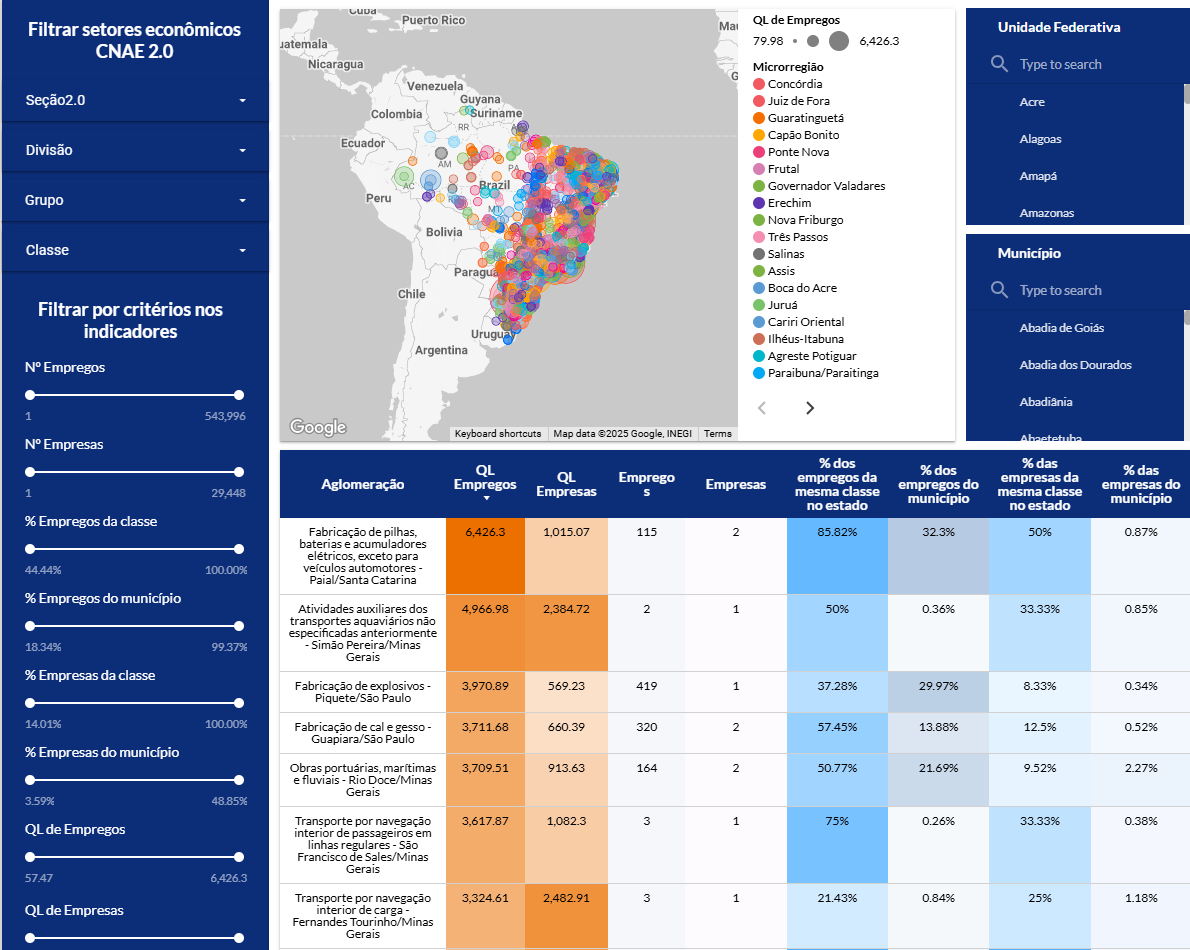
\includegraphics[width=0.9\textwidth]{images/2d_ObsEPTITAU.png}
	\caption{Painel interativo do Observatório EPT Fundação Itaú, 
		com filtros por CNAE, mapa de distribuição e tabela de aglomerações produtivas locais.}
	\label{fig:obs_ept}
\end{figure}

\textbf{Elementos do painel interativo}  
O Observatório EPT apresenta a informação por meio de um painel em ambiente 
Looker Studio, composto por quatro partes principais que funcionam de forma 
integrada: filtros, mapa, tabela e seleção territorial.  

\textbf{Filtros principais.} Localizados no lado esquerdo, permitem refinar a análise 
por \underline{CNAE 2.0} em diferentes níveis (Seção, Divisão, Grupo ou Classe) e 
aplicar controles deslizantes (\emph{sliders}) para limitar o número mínimo de empregos, 
de empresas ou o valor do quociente locacional. Esses filtros ajudam o usuário a 
focar em setores e atividades com maior peso relativo em uma região.  

\textbf{Mapa.} A parte superior do painel mostra a distribuição geográfica dos setores 
selecionados, por município ou microrregião. A cor dos polígonos representa a 
intensidade do indicador (empregos, empresas ou QL), permitindo visualizar 
rapidamente os pontos de maior concentração.  

\textbf{Tabela.} A parte inferior apresenta a lista detalhada das aglomerações 
produtivas locais (setor + território), que pode ser ordenada pelo usuário. Entre as 
colunas estão: número de empregos, número de empresas, quociente locacional 
para empregos e para empresas, além da participação percentual do setor no 
município e no estado.  

\textbf{Seleção territorial.} No lado direito, há menus suspensos que permitem escolher 
a unidade da federação (UF) ou o município de interesse. A escolha atualiza o mapa 
e a tabela de forma automática, facilitando o recorte espacial.  

Esses elementos, usados em conjunto, permitem ao analista explorar de forma 
interativa quais setores produtivos apresentam maior concentração regional, onde 
estão localizados e como se comparam em termos de emprego e empresas.


\subsection{Arranjos Produtivos Locais Ocupacionais (APLO)}

Apresentamos uma abordagem baseada em ocupações (CBO) para a identificação de arranjos produtivos locais, utilizando microdados da RAIS para os anos de 2023 e 2024. A metodologia estima a especialização relativa de ocupações nos níveis municipal, regional e estadual. Por se apoiar diretamente na estrutura ocupacional, esta abordagem permite associar os arranjos identificados aos cursos técnicos do Catálogo Nacional de Cursos Técnicos (CNCT), oferecendo subsídios para o planejamento da oferta de EPT alinhada ao perfil produtivo dos territórios.

\textbf{Identificação de Ocupações com Especialização Local}

A identificação das ocupações com possível base produtiva local é realizada a partir da base RAIS, utilizando códigos CBO de 4 dígitos (famílias ocupacionais) e aplicando a métrica de quociente locacional (QL), também conhecida como \textit{Revealed Comparative Advantage} (RCA). O QL compara a participação de uma ocupação no total de vínculos formais do município com a respectiva participação da mesma ocupação no total de vínculos do Brasil:

\[
QL_{m,o} = \frac{\frac{E_{m,o}}{E_m}}{\frac{E_{br,o}}{E_{br}}}
\]

Onde:

\begin{itemize}
	\item $E_{m,o}$ = número de vínculos para ocupação $o$ no município $m$
	\item $E_m$ = total de vínculos no município $m$
	\item $E_{br,o}$ = vínculos para ocupação $o$ no Brasil
	\item $E_{br}$ = total de vínculos no Brasil
\end{itemize}

Considera-se que um município tem especialização local em determinada ocupação se $QL_{m,o} \geq 1$, desde que haja também um mínimo de 30 vínculos registrados para aquela ocupação no município. A análise é aplicada para os anos de 2023 e 2024 e, como critério adicional de robustez, considera-se apenas os casos em que a ocupação satisfaz os critérios em ambos os anos (persistência).

\vspace{1em}

\textbf{Métricas de Diversidade, Ubiquidade e Complexidade}

A partir da matriz binária de presença de ocupações com especialização local ($QL_{m,o} \geq 1$), são extraídas medidas de estrutura da base produtiva local. Essas métricas complementam a identificação de APLs e ajudam a caracterizar os territórios e as ocupações:

\begin{itemize}
	\item \underline{Diversidade municipal}: mede a variedade de especializações ocupacionais observadas em cada município. Utilizamos duas métricas:
	\begin{itemize}
		\item \textit{Índice de Herfindahl-Hirschman (HHI)} — indica concentração; valores altos sugerem baixa diversidade.
		\item \textit{Entropia de Shannon} — mede dispersão; valores altos indicam maior diversidade.
	\end{itemize}
	
	\[
	HHI_m = \sum_o \left(\frac{E_{m,o}}{E_m}\right)^2
	\qquad\text{e}\qquad
	Shannon_m = -\sum_o \left(\frac{E_{m,o}}{E_m} \cdot \log \left( \frac{E_{m,o}}{E_m} \right) \right)
	\]
	
	\item \underline{Ubiquidade ocupacional}: número de municípios nos quais a ocupação apresenta especialização ($QL \geq 1$).
	
	\item \underline{Complexidade ocupacional}: média da diversidade (HHI ou Shannon) dos municípios onde a ocupação aparece com $QL \geq 1$.
	
	\item \underline{Complexidade municipal}: média da ubiquidade das ocupações especializadas naquele município.
\end{itemize}

\textbf{Correspondência das Ocupações (CBO) com Cursos Técnicos (CNCT)}

Para cada ocupação com especialização local identificada no passo anterior, realiza-se uma correspondência com cursos técnicos do Catálogo Nacional de Cursos Técnicos (CNCT), utilizando métodos de similaridade semântica entre descrições de cursos e ocupações.
 A correspondência é baseada em embeddings gerados a partir de modelos de linguagem e envolve múltiplos critérios (semântica, TF-IDF, vetores densos), resultando em uma pontuação final de similaridade ($\text{final\_score}$). Para cada ocupação (CBO de 6 dígitos), são selecionados os 20 cursos mais próximos. Em seguida, agregamos esses resultados para o nível de família ocupacional (CBO de 4 dígitos), retendo os 5 cursos com maior pontuação média. Essa etapa produz, para cada ocupação com RCA ≥ 1, uma lista dos cursos técnicos mais coerentes com seu perfil, permitindo inferir quais formações técnicas seriam mais adequadas ao perfil produtivo local.


\textbf{Correspondência das Ocupações (CBO) com Cursos Técnicos (CNCT)}

Para cada ocupação com especialização local identificada no passo anterior, realiza-se uma correspondência com cursos técnicos do Catálogo Nacional de Cursos Técnicos (CNCT), utilizando métodos de similaridade semântica entre descrições de cursos e ocupações.
A correspondência é baseada em embeddings gerados a partir de modelos de linguagem e envolve múltiplos critérios (semântica, TF-IDF, vetores densos), resultando em uma pontuação final de similaridade ($\text{final\_score}$). Para cada ocupação (CBO de 6 dígitos), são selecionados os 20 cursos mais próximos. Em seguida, agregamos esses resultados para o nível de família ocupacional (CBO de 4 dígitos), retendo os 5 cursos com maior pontuação média.
Essa etapa produz, para cada ocupação com RCA ≥ 1, uma lista dos cursos técnicos mais coerentes com seu perfil, permitindo inferir quais formações técnicas seriam mais adequadas ao perfil produtivo local.


\textbf{Integração com Dados de Matrícula do Censo Escolar}

Os cursos técnicos identificados como relevantes para os APLs são cruzados com os dados de matrícula disponíveis no Censo Escolar de 2023 e 2024. A comparação é realizada por estado (UF) e, quando possível, desagregada por curso e por dependência administrativa da escola (rede federal, estadual, municipal ou privada). Essa integração permite evidenciar eventuais lacunas entre a demanda ocupacional (inferida a partir dos APLs) e a oferta educacional atual. Embora a correspondência entre denominações de cursos possa não ser exata, utilizamos normalizações de texto para aproximar os nomes de cursos técnicos do CNCT com os registrados no Censo.


\newpage
\thispagestyle{empty}
\mbox{}



\newpage
\chapter{Oferta e Demanda conectada } 
\section{Metodología} 

Com o objetivo de buscar indícios de escassez de força de trabalho especializada, Nascimento (2011) utiliza dados do Caged e da Rais para verificar o comportamento mensal do mercado formal de trabalho para ocupações técnico-científicas. O autor se vale dos diferenciais salariais entre admitidos e desligados e da evolução das taxas de rotatividade como indicadores de escassez. Esse método foi replicado, com a mesma finalidade, por Sousa e Nascimento (2012), por Nascimento (2012) e por Lopes (2013).\footnote{Nascimento (2011) usa o método para identificar focos de escassez de pessoal técnico-científico no Brasil, enquanto que as três obras citadas na sequência o fazem para outros recortes. Sousa e Nascimento (2012) focam nas carreiras técnico-científicas no setor de telecomunicações no Brasil; Nascimento (2012) observam os postos de trabalho altamente demandantes de competências relacionadas à engenharia e ao design nas oito maiores regiões metropolitanas do país. Lopes (2013) estuda as profissões ligadas à engenharia e à arquitetura no estado do Mato Grosso.}
 
Adaptações no método podem, além de aprimorá-lo como ferramenta de identificação de focos de escassez de trabalho especializado, torná-lo útil à tomada de decisões relativas ao Propag. Tendo esse objetivo como bússola, organizamos indicadores, a partir de dados de emprego formal, para identificar sinais recentes de escassez em ocupações de nível técnico e priorizar cursos técnicos por Unidade da Federação (UF). O foco é prático: entregar aos gestores uma lista de cursos/áreas com demanda aquecida, conectada às metas 11a, 11b e 11c do PNE 2026–2035 e utilizável nas pactuações e no planejamento anual.

Para definir as ocupações de nível técnico a serem analisadas, recorremos à Classificação Brasileira de Ocupações (CBO). A CBO é o sistema de classificação que reconhece, nomeia e codifica os títulos e descreve as características das ocupações do mercado de trabalho brasileiro, sendo simultaneamente uma classificação enumerativa e descritiva. A versão em vigor (de 2002, mas periodicamente atualizada) contém as ocupações do mercado brasileiro, organizadas e descritas por grandes grupos (um dígito), subgrupos principais (dois dígitos), subgrupos (três dígitos), famílias (quatro dígitos) e as ocupações em si (cinco dígitos). Aquelas tomadas na análise são todas as do grande grupo 3, que corresponde aos técnicos de nível médio. A análise parte das ocupações com 3 ou 4 dígitos da CBO, a depender da densidade ocupacional observada.

A granularidade territorial das estimativas também precisa variar conforme a densidade populacional e econômica de cada UF. Nos estados com maior volume de admissões e desligamentos mensais, é possível desagregar a análise por região intermediária ou mesmo por região imediata, de acordo com classificação do IBGE. Já nos estados com menor dinamismo ocupacional, a análise se dará no âmbito estadual. Há, portanto, um trade-off entre desagregação territorial e desagregação ocupacional: é necessário haver variação suficiente nos fluxos mensais para que os indicadores gerados tenham validade estatística.

Para este relatório, nossa decisão foi apresentar resultados agregados para estados e o Distrito Federal, tomando a CBO a três dígitos. Com esse procedimento, pudemos elaborar uma plataforma interativa que fornece informações úteis para todas as UFs. 

Os dados necessários para o cálculo dos indicadores usados na análise são gratuitos e de fácil acesso a gestores estaduais. Estão disponíveis via o Programa de Disseminação de Estatísticas do Trabalho (PDET), do Ministério do Trabalho e Emprego (MTE). São dois os registros administrativos a que recorremos para o método ora proposto: o Cadastro Geral de Empregados e Desempregados (Caged) e a Relação Anual de Informações Sociais (Rais). 

O Caged registra, com periodicidade mensal, informações sobre admissão e desligamento nas firmas de todo o país. Permite observar os fluxos de geração e destruição de emprego ao longo do tempo. O Caged foi a principal fonte de dados utilizada, ao permitir calcular, mês a mês, os salários médios de admissão e de desligamento das variadas ocupações em um determinado recorte geográfico, bem como acompanhar a evolução do saldo líquido de horas contratadas. 

Já a Rais é um registro anual, no qual as firmas de todo o país prestam ao MTE informações detalhadas sobre cada um de seus colaboradores. Essas informações destinam-se a suprir as necessidades de controle da atividade trabalhista no país, prover dados para análises estatísticas acerca do mercado de trabalho e tornar disponível informações às entidades governamentais da área social. Por permitir observar os estoques de postos de trabalho ao final de cada ano, a Rais é a fonte de dados aqui utilizada para calcular os estoques de postos de trabalho. 

Valendo-se dessas duas fontes de dados (Caged e Rais), busca-se identificar os conjuntos de ocupações que apresentam maiores pressões de demanda. Para isso, recorre-se a um indicador da trajetória salarial. Este é o principal indicador utilizado na literatura para identificar desníveis entre oferta e demanda por trabalho especializado, embora informações assimétricas, seleções adversas e falhas de mercado decorrentes da rigidez dos salários, do poder dos sindicatos e de especificidades de cada nicho de mercado de trabalho acarretem limitações ao equilíbrio desses mercados pura e simplesmente pelo mecanismo de preços. 

A despeito dessas ressalvas, um indicador capaz de servir de proxy para pressão salarial é o mais útil como indicador de primeira ordem do aquecimento de uma ocupação. Observamos, então, o comportamento, ao longo do tempo, dos diferenciais salariais entre admitidos e desligados em cada ocupação. É de se esperar que o salário médio de desligados seja superior ao de admitidos para postos de trabalho que exijam as mesmas qualificações, pois entre os desligados há uma concentração maior de profissionais com mais tempo de carreira, enquanto que entre os admitidos a tendência é que haja uma concentração maior de profissionais mais jovens e menos experientes. Se esse diferencial apresenta uma tendência de diminuição ao longo do tempo (ou seja, se há um comportamento de catching up ao longo do tempo do salário médio de admissão em relação ao de desligamento), há uma sinalização de aquecimento do mercado por aquelas ocupações naquele recorte geográfico. 

Essa sinalização de aquecimento pode vir a indicar escassez relativa das ocupações analisadas, se os diferenciais salariais se tornarem favoráveis aos admitidos (contrariando a lógica geral de que tendem a ganhar menos do que quem foi desligado no mesmo período) ou se o comportamento de catching up vier acompanhado de taxas de rotatividade crescentes. A taxa de rotatividade entra aí como indicador complementar que, quando crescente em paralelo a uma trajetória salarial também crescente, reforça o indício de escassez relativa daquele subgrupo de ocupações na UF analisada. 

Como o objetivo desse exercício é oferecer informação a gestores estaduais sobre os cursos de EPT nos quais investir, utilizamos uma matriz de correspondência CBO→CNCT construída pela equipe (KENCHIAN et al, REF UNKNOWN), que associa famílias ocupacionais a cursos técnicos do Catálogo Nacional de Cursos Técnicos (CNCT). Com isso, a plataforma desenvolvida já dá a informação da demanda potencial por curso, não por subgrupo ocupacional.

O procedimento descrito abaixo resume o método ora apresentado e como que ele dialoga com outras partes deste relatório.

\textbf{(1) O que entra no modelo (fontes e recorte)}

\begin{itemize}
	\item Fontes: CAGED (fluxos mensais de admissões e desligamentos, com salários) e RAIS (estoque anual).
	\item Unidade de análise: UF × curso técnico (CNCT) × mês, com mapeamento CBO→CNCT já incorporado às bases de trabalho.
	\item Período: 2020–2024 (séries mensais).
	\item Padronização de salários: ajuste para 44h semanais e uso de média móvel de 12 meses para suavizar oscilações.
	\item Resultado: um painel mensal que permite comparar cursos/áreas dentro da UF e ao longo do tempo, com métricas homogêneas.
\end{itemize}

\textbf{(2) Sinais de escassez utilizados}

O painel mostra, para cada UF × curso (CNCT) × mês, os seguintes dados:

\begin{enumerate}
	\item Valorização salarial relativa (sinal de aquecimento): diferença entre salários médios de admitidos e desligados, trabalhada em média móvel 12 meses.
	\item Rotatividade: soma de admissões e desligamentos em relação ao estoque estimado, também em média móvel 12 meses.
	\item Intensidade do curso na UF: participação do curso no estoque estadual (para distinguir áreas relevantes de nichos residuais).
\end{enumerate}

Filtro mínimo de fluxo: para evitar ``falsos positivos'' em séries muito rarefeitas, só são consideradas observações com mais de 30 admissões no mês.

\textbf{(3) Classificação do ``grau de escassez''}

Combinam-se os três sinais em uma tipologia simples (rótulos prontos para uso em painéis/relatórios):

\begin{itemize}
	\item 3 – Alerta de escassez: valorização alta e rotatividade ao menos mediana e intensidade relevante (acima de cortes pré-definidos), com fluxo > 30;
	\item 2 – Tendência de escassez: combinações intermediárias dos três sinais, com fluxo > 30;
	\item 1 – Estável: valorização moderada/baixa ou intensidade pequena, com fluxo > 30;
	\item 0 – Sem indício: valorização baixa;
	\item 99 – Sem fluxo suficiente: não passou no filtro > 30.
\end{itemize}

Essa rotulagem entrega ao gestor uma leitura rápida do ``onde priorizar'' dentro de cada UF.

\textbf{(4) Do ``sinal'' à priorização de cursos (CNCT)}

A leitura gerencial é direta: cursos/áreas classificados como 3 (alerta) ou 2 (tendência) formam a carteira prioritária para expansão e/ou readequação de oferta (por rede e tipo de curso). Essa carteira é o insumo para:

\begin{itemize}
	\item discutir metas anuais de vagas/matrículas por tipo de oferta (integrado, concomitante, subsequente e EJA-EM+EPT),
	\item dialogar com outras redes atuantes na UF (federal, estadual/distrital, municipal, privada/Sistema S), com vistas a estabelecer parcerias que evitem sobreposição de esforços, e
	\item dimensionar custos em dois cenários (com e sem Propag), conforme discussão em outros capítulos deste relatório.
\end{itemize}

\textbf{(5) Como isso conversa com as metas 11a, 11b e 11c}

\begin{itemize}
	\item 11a (razão EPT/EM = 50\%): a carteira priorizada indica onde expandir para elevar o numerador (EPT técnica + EJA-EM com EPT), respeitando as projeções do denominador (EM total projetado, sem dupla contagem).
	\item 11b (subsequentes +50\%): as áreas com sinal ``adulto/ocupacional'' (muita movimentação e valorização) alimentam a trilha de cursos subsequentes, foco direto da meta.
	\item 11c (≥25\% da EJA articulada à EPT): priorizam-se cursos com empregabilidade clara para públicos EJA, elevando a proporção articulada à EPT.
\end{itemize}

Em todos os casos, as projeções demográficas e a distribuição por rede (ecossistema da UF) são consideradas nos volumes/cronogramas, mas a identificação de prioridades nasce do sinal empírico descrito acima.

Tal como já implementado na plataforma disponibilizada, o painel gerado a partir do método aqui descrito já é de grande valia para o gestor. Ele pode ser ainda customizado para as necessidades de cada UF. Pode ainda vir a ser aperfeiçoado com a inclusão de indicadores alternativos que podem ser úteis para enriquecer o diagnóstico — por exemplo, podemos usar o coeficiente locacional (CL) para levantar informações sobre especialização regional e usar o saldo líquido de horas contratadas como indicador complementar de aquecimento e substituto da taxa de rotatividade. Essas abordagens não estão ainda implementadas, portanto não compõem os cálculos da versão atualmente disponibilizada do painel. Podem, contudo, ser incorporadas como módulos opcionais em edições futuras, sem alterar a lógica central aqui descrita.\footnote{Bastante utilizado em estudos regionais e urbanos, o coeficiente locacional “ajuda a entender o grau relativo de concentração de um determinado fenômeno em cada região de um país” (Maciente, Pereira e Nascimento, 2013, p. 430). No caso ora em análise, o fenômeno seriam os postos de trabalho relacionados a um determinado grupo ocupacional.Tambem, veja o Capítulo 4 desse relatorio}

Em resumo, o método aqui descrito vale-se da Rais e do Caged para, a partir da CBO e do CNCT, produzir três sinais simples (valorização, rotatividade e intensidade), um filtro mínimo de fluxo e uma classificação gerencial que aponta onde a UF ganha mais ao expandir a EPT — e como isso ajuda a cumprir as metas 11a, 11b e 11c do novo PNE. Extensões como coeficiente locacional e saldo de horas são opcionais para versões futuras, não alterando a entrega principal aos gestores.

A despeito dessas vantagens, o método não pode e não deve ser usado como única fonte de informação no processo de tomada de decisões acerca das vagas a serem abertas. Suas limitações mais evidentes passam por:

\begin{itemize}
	\item os indicadores propostos olham para o passado. Por mais que o Caged forneça dados de fluxos mensais de emprego e o MTE consiga divulgar atualizações com relativa rapidez, os cursos e as vagas que vierem a ser abertos a partir dos indicadores daí gerados baseiam-se em fotografias tiradas do mercado formal de trabalho no passado – que não necessariamente se perpetuarão no futuro.
	\item os indicadores propostos não alcançam o trabalho informal. Dados do Caged e da Rais referem-se exclusivamente a postos de trabalho ocupados por celetistas e estatutários. Vínculos não formais não são captados por esses registros administrativos, razão pela qual há que
	\item os indicadores propostos perdem qualidade à medida que são desagregados.
\end{itemize}

O planejamento de metas de formação profissional técnica requer estimativas robustas sobre a demanda por ocupações técnicas no território. Para isso, este relatório propõe um método de estimação da demanda com base em dados históricos de mercado de trabalho, em uma abordagem retrospectiva (\textit{backward-looking}), centrada na identificação de sinais persistentes de escassez relativa de profissionais.

A abordagem é considerada \textit{backward-looking} porque se ancora na observação de trajetórias passadas de dois indicadores derivados de microdados do Caged (fluxos) e da Rais (estoque): i) o diferencial salarial entre admitidos e desligados; e ii) a taxa de rotatividade. A convergência ou inversão do diferencial salarial, combinada a uma rotatividade elevada e persistente, sugere desequilíbrios entre oferta e demanda por determinada ocupação, os quais podem justificar intervenções formativas para suprimento dessa escassez. É recomendável, sem embargo, que, adicionalmente à plataforma viabilizada com este método, o gestor busque igualmente indicadores que incorporem mudanças prospectivas nos padrões de emprego.

As limitações apontadas não invalidam as vantagens já enumeradas do painel disponibilizado. Com efeito, ele permite construir um retrato dinâmico da demanda por profissionais técnicos, ajustável às condições econômicas e institucionais locais. Trata-se de uma entrega concreta e objetiva para gestores estaduais, que compreende:

\begin{enumerate}
	\item Painel/planilha com a tipologia (0/1/2/3) por UF × curso × mês, já em percentis e com filtro de fluxo aplicado;
	\item Lista priorizada de cursos/áreas por UF para pactuação (com indicação do tipo de oferta e redes preferenciais);
	\item Insumos para metas anuais (vagas/matrículas) e para os dois cenários financeiros (com/sem Propag), a serem detalhados nos capítulos seguintes.
\end{enumerate}

\newpage
\input{sections/part1/Resultados}
\clearpage

\newpage
\thispagestyle{empty}
\mbox{}


\part{Apêndice}


\newpage
\thispagestyle{empty}
\mbox{}



\newpage
\backgroundbarvisiblefalse  % Turn off the vertical bar for Annex
\backgroundtitlevisiblefalse % Turn off the rotated text
\chapter{Normativas e relacionados}
\section*{Lei Complentar 212  e Decreto 12.433}

In faucibus orci luctus et ultrices posuere cubilia curae; Aliquam nunc ipsum,
sollicitudin ut tempus consectetur, fermentum at lectus.


\section*{Notas Técnicas publicadas}

In faucibus orci luctus et ultrices posuere cubilia curae; Aliquam nunc ipsum,
sollicitudin ut tempus consectetur, fermentum at lectus.
%https://www.gov.br/fazenda/pt-br/acesso-a-informacao/acoes-e-programas/propag-renegociacao-de-dividas-de-estados-e-distrito-federal-com-a-uniao


\section*{Apresentações publicadas}

In faucibus orci luctus et ultrices posuere cubilia curae; Aliquam nunc ipsum,
sollicitudin ut tempus consectetur, fermentum at lectus.

\section*{Legislação Minas Gerais}

In faucibus orci luctus et ultrices posuere cubilia curae; Aliquam nunc ipsum,
sollicitudin ut tempus consectetur, fermentum at lectus.

\section*{Legislação Goiás}

In faucibus orci luctus et ultrices posuere cubilia curae; Aliquam nunc ipsum,
sollicitudin ut tempus consectetur, fermentum at lectus.


\newpage
\thispagestyle{empty}
\mbox{}

\newpage
\listoffigures
\listoftables
%----------------------------------------------------------------------------------------
\newpage
\printbibliography[title={Referências}]
\clearpage

\newpage
\thispagestyle{empty}
\mbox{}

\newpage
\thispagestyle{empty}
\mbox{}

\backcover


\end{document}
